\documentclass[french, a4paper, 12pt]{report}
\usepackage[margin=2.5cm]{geometry}
\usepackage[utf8]{inputenc}
\usepackage[frenchb]{babel}
\usepackage[T1]{fontenc}
\usepackage{babel}
\usepackage{graphicx}
\usepackage{lettrine}
\usepackage{lmodern}
\usepackage{eso-pic}
\usepackage{tabularx}
\usepackage{titlesec}
\usepackage{colortbl}
\usepackage{xcolor}
\usepackage{setspace}
\usepackage{tikz}
\usepackage{hyperref}
\usepackage{stmaryrd}
\usepackage{subfig}
\usepackage{graphicx} 
\usepackage{caption}
\usepackage{mwe}
\usepackage{lipsum}
\usepackage{filecontents}
\usepackage{wrapfig}
\usepackage{url}
\hypersetup{
    colorlinks=true,
%     linkcolor=blue,
    citecolor=black,
    filecolor=black,
    linkcolor=black,
    urlcolor=black
}


\definecolor{olivegreen}{rgb}{0,0.5,0}

\titleformat{\chapter}[hang]{\bf\LARGE}{\thechapter}{0pc}{ - }
\titleformat{\section}[hang]{\bf\Large}{\thesection}{0pc}{ - }
\titleformat{name=\chapter,numberless}[hang]{\bf\LARGE}{}{0pc}{}
\titleformat{name=\section,numberless}[hang]{\bf\Large}{\thesection}{0pc}{}
%%%%%%%%%%%%%%%%%%%%%%%%%%%%%%%%%%%%%%%%%%%%%%%%%%%%%
%%%%%%%%%%%%% PROJECT TITLE%%%%%%%%%%%%%%%%%%%%%%%%%

\title{Mémoire fin d'étude }


%%%%%%%%%%%%%%%%%%%%%%%%%%%%%%%%%%%%%%%%%%%%%%%%%%%%




\begin{document}
%%%%%%%%%%%%%%%%%%
%%% First page %%%
%%%%%%%%%%%%%%%%%%

\begin{titlepage}
\begin{center}

\begin{figure}[!htb]
\minipage{0.25\textwidth}
  
\includegraphics[width=\linewidth]{images/parisNanterre-logo}
\endminipage\hfill
\minipage{0.2\textwidth}
  
\includegraphics[width=\linewidth]{images/logo_afia_2x.png}
\endminipage\hfill
\minipage{0.2\textwidth}%
  
\includegraphics[width=\linewidth]{images/datategy.png}
\endminipage
\end{figure}
\vspace{1cm}
{\Large Mémoire de fin d'étude Master 2 MIAGE}\\[0.5cm]



% Title
\rule{\linewidth}{0.5mm} \\[0.4cm]
{ \huge \bfseries Quel est l'impact de la visualisation du Big Data sur les smart cities? \\[0.4cm] }
\rule{\linewidth}{0.5mm} \\[1.5cm]
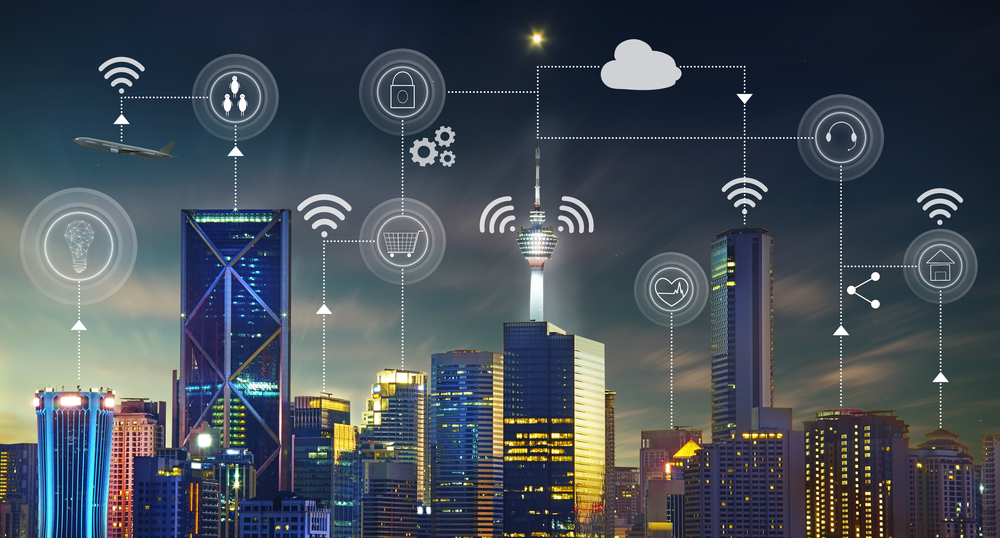
\includegraphics[width=1\textwidth]{images/Smart-City.jpg}\\[1cm]
% Author and supervisor
\noindent
\begin{minipage}{0.4\textwidth}
  \begin{flushleft} \large
    \emph{Étudiant :}\\
    Hani \textsc{Abdulwahab}
  \end{flushleft}
\end{minipage}%
\begin{minipage}{0.4\textwidth}
  \begin{flushright} \large
    \emph{Encadrants :} \\
    Mme.~Sonia \textsc{GUEHIS}\\
    M.~Mehdi \textsc{CHOUITEN }

  \end{flushright}
\end{minipage}

\vfill

% Bottom of the page
{\large Version 0.1 du\\ \today}

\end{center}
\end{titlepage}

\tableofcontents
\listoffigures
\chapter*{Remerciements}

\chapter*{Introduction}
\addcontentsline{toc}{chapter}{Introduction}
Une ville intelligente idéale est une ville où l’on peut mener une vie saine et agréable, avec à disposition des moyens de transport fiables. Une ville intelligente, en tant qu’organisme vivant, vérifie ses fonctions vitales, s’ajuste et se maintient saine, minimisant ainsi les inconvénients de l’urbanisation. Loin des embouteillages, des pénuries de logements, des concentrations malsaines de poussière fine, des centres-villes surpeuplés, des structures sociales en ruine et du bruit.
L'expansion du Big Data et l'évolution des technologies de l'Internet des objets (IoT) ont joué un rôle important dans la faisabilité des initiatives de ville intelligente. Les mégadonnées offrent aux villes la possibilité d’obtenir des informations précieuses à partir d’un grand nombre de données recueillies auprès de diverses sources, et l’Internet des objets permet l’intégration de capteurs, d’identification par radiofréquence et de Bluetooth dans un environnement réel utilisant des services hautement interconnectés. La combinaison de l'IoT  et du Big Data est un domaine de recherche inexploré qui a apporté de nouveaux défis intéressants pour atteindre l'objectif des futures villes intelligentes. Ces nouveaux défis se concentrent principalement sur des problèmes liés aux technologies qui permettent aux villes d’actualiser la vision, les principes et les exigences des applications des villes intelligentes en réalisant les principales caractéristiques de l’environnement intelligent.
Les smart cities sont le futur des grandes villes et les entreprises doivent décider de comment gérer les données et comment permettre à ses parties prenantes de prendre des décisions. 
%La flexibilité et la rapidité seront les critères qui obligeront ces entreprises à tendre vers la visualisation Big Data.
Les données sont toujours plus nombreuses, plus complexes, plus variées et donc plus volumineuses, et plus particulièrement dans le cas des Smart Cities. 
Comment les analyser et en tirer profit pour prendre la meilleures décision au sein d’une entreprise et stimuler sa croissance ? 
%Pour répondre à cette problématique “Une image vaut mieux que mille mots”.
La visualisation de données est la présentation de données dans un format graphique. Il permet aux décideurs de voir les analyses présentées de manière visuelle, afin de pouvoir comprendre mieux et d’identifier de nouveaux modèles. 
Pour la business intelligence, la visualisation des données est très utile. Au lieu de parcourir un rapport comportant des centaines de lignes, un utilisateur professionnel peut simplement consulter un graphique.
Pour les Smart cities, elles apparaissent comme une stratégie de gestion de la performance urbaine. Pour ce processus, il est nécessaire de visualiser un grand nombre de paramètres, souvent en temps réel. 
La visualisation des données est devenue un centre d'intérêt pour la recherche, les industries, les gouvernements et les autres organisations pour améliorer la mobilité, l'efficacité énergétique, la gestion des déchets et l'administration publique d'une ville intelligente. Les exigences du Big Data, les volumes croissants, les formats et normes de qualité variables, présentent des défis pour la gestion, le stockage, la visualisation et l'analyse des données, telles que la Geo-Visualisation et la Visual Analytics des données géospatiales. Celles-ci sont collectées dans une ville intelligente et permettent de décrire le potentiel de telles techniques. Cela aidera à mieux comprendre le système urbain et à permettre le développement durable des villes futures en améliorant les interactions humaines avec les données géospatiales.

Dans le cadre de mon Master M2 MIAGE à l’Université Paris Nanterre, j’ai souhaité réaliser cette mémoire sur l'impact de la visualisation du Big Data sur les smat cities. 
%En effet, j’ai effectué au cours de mes études d’ingénieur en Télécommunication un mémoire sur la reconnaissance sonore qui permettait de visualiser le son avec une image. Ce mémoire m’a fait découvrir l’intérêt de la visualisation. 
Actuellement, le contexte des villes modernes souhaitant devenir des villes intelligentes met en valeur la visualisation comme moyen d’analyse des données. L’enjeu est important pour des entreprises comme Datategy où j’effectue mon alternance en tant que développeur web front-end. J’ai eu de nombreuses tâches sur la visualisation du Big Data dans le cadre d’une Smart City. Les réalisations effectuées grâce à la visualisation du Big Data, l’utilisation de différentes techniques  et outils m’intéressent particulièrement. 

Dans un premier temps, la définition théorique de la ville intelligente sera présenté. Cette définition se veut être un idéal vers lequel la ville intelligente veut tendre. L’impact de l'évolution des Smart Cities sur les domaines de l’économie, de la gouvernance, de l’environnement, de la mobilité et de la démographie seront analysés. Puis, le rôle de la technologie dans les Smart Cities telles que les données numériques (Big Data) et l’Internet of Things (IoT) sera abordé. Puis, la visualisation du Big Data, ses défis ainsi que les techniques et les outils de visualisation de données sera présentés. 
Dans un second temps, la réalisation d’une étude comparative entre les différentes techniques et outils présentés dans le chapitre précédent. 
Dans un troisième temps, nous décrirons un cas pratique :  la visualisation du Big Data chez Datategy. 
Finalement, un bilan professionnel et personnel sera présenté. 

\chapter{Smart city  et  visualisation du Big Data}
\section{Smart city}
\subsection{Définition de la ville intelligente}
\subsubsection{Historique:}
La croissance des villes depuis la révolution industrielle a atteint des niveaux sans précédent. 
%La division de la population des Etats-Unis a estimé qu'en 2016, 54,5\% de la population mondiale vivait dans des zones urbaines et qu'en 2050, ce nombre atteindrait 67\% \cite{0}. 
Cette croissance considérable de la population urbaine nécessitera d’importants développements d’infrastructures urbaines pour faire face à la demande de ses habitants. Il ne fait aucun doute que les villes sont des systèmes complexes et que la croissance urbaine rapide engendre des embouteillages, une pollution et une inégalité sociale croissante. Ceux-ci peuvent transformer la ville en un point de convergence de nombreux risques (économiques, démographiques, sociaux et environnementaux). Cela pourrait sérieusement dépasser leur capacité à fournir des services adéquats à leurs citoyens \cite{1}. Cependant, des villes bien gérées peuvent offrir de multiples avantages aux personnes qui y vivent car elles permettent de réaliser des économies d’échelle en partageant des commodités telles que les transports, les installations de sport et de divertissement, les services aux entreprises, le haut débit, etc.
Depuis les années 1990, les gouvernements et les chercheurs utilisent le terme « villes intelligentes » comme un label de mode ou pour aider certaines villes à se distinguer et à se promouvoir comme innovantes. Être une ville intelligente est une aspiration pour certaines villes qui ont élaboré des plans à long terme afin d’atteindre cet objectif. Le terme ville intelligente est considéré comme un anthropomorphisme (attribution de caractéristiques humaines à la ville), car il repose sur la capacité de la ville à détecter et à relever ses défis de manière intelligente, en utilisant une intelligence naturelle et artificielle intégrée aux systèmes d’information de la ville \cite{2}.
\subsubsection{Définition:}
De nombreuses études ont tenté de définir le concept de ville intelligente, mais le défi reste difficile à relever. C’est un concept multidisciplinaire et il est difficile de définir le terme « intelligent ». Les premières tentatives de définition du concept ont été axées sur l'intelligence des technologies de l'information pour la gestion de diverses fonctions de la ville \cite{3}. 
Dernièrement, les études ont élargi leur champ d'action en incluant les résultats de la ville intelligente tels que la durabilité, la qualité de vie et les services aux citoyens.
L'évaluation du niveau d'intelligence des villes est également devenue importante pour les chercheurs et les responsables gouvernementaux. Ils ont développé des classements prenant en compte des variables telles que l'économie, les infrastructures, l'innovation, la qualité de vie, les transports, le développement urbain, etc. \cite{4}.
Malgré la vaste littérature sur les villes intelligentes, il existe plus de trente définitions du terme. Ils abordent des aspects différents, mais pertinents, notamment la construction de ces villes \cite{5}. 
Il ne fait aucun doute qu'une ville intelligente est un concept multidisciplinaire qui englobe non seulement son infrastructure informatique, mais également sa capacité à gérer les informations et les ressources pour améliorer la qualité de vie de ses habitants. L'utilisation de la technologie de l'information est considérée comme un facteur clé de l'intelligence d'une ville, car elle peut détecter, surveiller, contrôler et communiquer la plupart des services de la ville tels que les transports, l'électricité, le contrôle de l'environnement, la lutte contre la criminalité, les urgences sociales, etc \cite{6}.
\subsection{Étapes pour la mise en œuvre de projets de ville intelligente}

La mise en œuvre réussie d'un projet de ville intelligente nécessite la mise au point d'un système numérique capable de gérer et de visualiser les données géospatiales dans un environnement convivial. Le système d'information géographique (SIG) offre des fonctionnalités avancées et convivial pour les projets de ville intelligente.
Le concept de « ville intelligente » vise à développer un système complet qui utilise des données géospatiales pour améliorer la compréhension des systèmes urbains complexes et pour améliorer l’efficacité et la sécurité de ces systèmes. 
Ces données géospatiales concernent :
\begin{itemize}
\item \textbf{} L’environnement urbain construit tel que les infrastructures, les bâtiments et les espaces publics.
\item \textbf{} L’environnement naturel tel que la biodiversité, les espaces verts, la qualité de l’air, le sol et l’eau.
\item \textbf{} Les services urbains tels que les transports, les déchets municipaux, l’eau, l’énergie, la santé et l’éducation. 
\end{itemize} 
Le concept de ville intelligente vise également à transformer la gestion des villes «en silo» en un système «partagé» impliquant les acteurs urbains dans la conception, la réalisation et l’évaluation de projets urbains.
\begin{figure}[!ht]
    \centering
    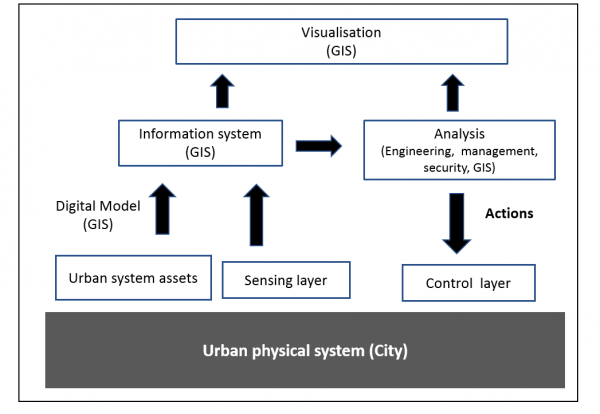
\includegraphics[height=8cm]{images/Steps.png}
    \scriptsize{source :}
    \caption{Étapes pour la mise en œuvre d’un projets de ville intelligente}
    \label{fig:2.1}
\end{figure}
Figure~\ref{fig:2.1} inclut la construction du modèle numérique urbain, la collecte de données à l'aide de la couche de détection, puis l'analyse des données, la visualisation interactive des données et le contrôle du système. Le SIG joue un rôle dans ces étapes, comme décrit ci-dessous. 

\subsubsection{1. Construction du modèle de ville intelligente:}
La première étape de la mise en œuvre d’un projet de ville intelligente concerne la construction du modèle numérique urbain qui décrit les composants des environnements urbains et naturels construits. Le modèle numérique fournit pour chaque composant urbain la géolocalisation et les caractéristiques (attributs). Les SIG sont généralement utilisés pour la construction du modèle numérique de «composants horizontaux» urbains tels que les réseaux urbains, les installations de transport et l’environnement naturel, tandis que la modélisation des données du bâtiment (BIM) est utilisée pour la description de «composants verticaux» tels que les bâtiments. La combinaison des SIG et du BIM fournit un outil puissant pour la construction du modèle numérique urbain avec des données géoréférencées et la visualisation de ces données dans un environnement convivial.

\subsubsection{2. Couche de détection:}
La deuxième étape d’un projet de ville intelligente concerne la construction de la couche de détection qui transfère les données d’exploitation urbaine au système d’information de la ville intelligente. Cette couche comprend des capteurs utilisés pour la surveillance des réseaux et infrastructures urbains. Les données pourraient également être enrichies d'images, de vidéos et de fichiers audio, ce qui aboutirait à la construction de mégadonnées urbaines. Par exemple le système d'eau potable utilise des lecteurs de compteurs automatiques (AMR) pour enregistrer la consommation d'eau, des capteurs de pression pour enregistrer la pression de l'eau et des dispositifs de contrôle de la qualité de l'eau permettant de suivre la qualité de l'eau (turbidité, pH, chlore, conductivité). Le système de drainage utilise des capteurs pour surveiller le niveau et le débit d'eau, la qualité de l'eau (turbidité, température, pH, etc.) et le matériel de pompage. Il permet une détection précoce des inondations et des défauts dans les équipements de pompage. Le réseau électrique utilise des capteurs pour mesurer la tension électrique, le courant et la fréquence. Il permet une détection précoce des défauts du réseau électrique. Le système de chauffage urbain est surveillé par des capteurs pour enregistrer la température, la pression et le débit du fluide, ainsi que l'état de la vanne. Il permet la détection précoce des pannes et l'amélioration des performances du système. Le SIG offre la possibilité de visualiser le système de surveillance ainsi que les caractéristiques et l’état des capteurs. Il offre également la possibilité de visualiser des données historiques et en temps réel sur des cartes SIG.
\subsubsection{3. L'analyse des données:}
La troisième étape de la mise en œuvre d'un projet de ville intelligente concerne le développement d'un environnement analytique, qui transforme les données en temps réel améliorant la sécurité, l'efficacité et la qualité des systèmes urbains. L'environnement analytique comprend des logiciels d'ingénierie, de gestion et de sécurité pour les systèmes urbains, ainsi que des outils numériques avancés tels que l'intelligence artificielle (IA). Dans les projets de ville intelligente, les SIG fournissent des outils pour (i) l’analyse de données géospatiales (traitement géométrique, modèles de grille), (ii) l’analyse spatio-temporelle, (iii) les statistiques spatiales (autocorrélation spatiale et modèle de régression), (iv) l’analyse de surface (analyse de la forme et du flux de surface, méthodes de maillage et d'interpolation) et (v) analyse de localisation (calcul du plus court chemin, localisation de l'installation).

\subsubsection{4. Visualisation interactive des données:}
La visualisation interactive des données permet aux utilisateurs d’interagir avec les composants de la ville intelligente et les parties prenantes (Skateholder) dans un environnement convivial. Les applications Web sont utilisées pour créer cet environnement interactif. L'utilisation de fenêtres contextuelles HTML permet aux utilisateurs d'accéder à du contenu Web, tel que des graphiques référencés par des URL. L'environnement graphique SIG interactif permet la visualisation de composants urbains et de cartes de capteurs. Les utilisateurs et les gestionnaires peuvent utiliser ces cartes pour accéder aux données statiques et dynamiques concernant les systèmes urbains ainsi que pour mettre à jour les données.

\subsubsection{5. Couche de contrôle}
L'analyse des données en temps réel et des données historiques donne lieu à des commandes pour une gestion optimale et sécurisée des systèmes urbains. Ces commandes sont transmises à la couche de contrôle, qui comprend différents dispositifs électroniques tels que des vannes intelligentes, des pompes, des moteurs, des commutateurs, des disjoncteurs et des serrures. Le système SIG permet une visualisation en temps réel de ces appareils ainsi que de leur statut. Il pourrait également visualiser les erreurs dans la commande de l'appareil.
%%%%%%%%%%%%%%%%%%%%%%%%%%%%%%%%%%%%%%%%%%%%%%%%%%%%%%%%%%%%%%%%%%%%%%%
\subsection{Avantages et opportunités}
Les avantages d’une ville intelligente sont notamment les suivants [9] :
\begin{itemize}
\item \textbf{}Amélioration de la qualité de vie des citoyens.
\item \textbf{}Mise en place d’une gestion intelligente des infrastructures et des ressources naturelles.
\item \textbf{}Utilisation efficace des ressources avec les systèmes technologiques tels que la planification des ressources d'entreprise (ERP) et le système d'information géographique (SIG) [9].
\item \textbf{}Meilleure qualité de vie pour les citoyens : grâce à des services plus rapides, moins coûteux en temps et en énergie, à une meilleure planification des espaces et des lieux de vie et de travail, à des transports plus efficaces et à la disponibilité des informations concernant la ville pour les citoyens. 
\item \textbf{}Niveaux plus élevés de transparence et d’ouverture : le partage des données et des ressources, la transparence de l'information pour toutes les personnes impliquées encourage la collaboration et la communication entre entités et la création de plus de services et d'applications améliorant davantage la ville intelligente.
\end{itemize}
%%%%%%%%%%%%%%%%%%%%%%%%%%%%%%%%%%%%%%%%%%%%%%%%%%%%%%%%%%%%%%%%%%%%%%%
\section{Le rôle de la technologie dans les smart cities}
\subsection{Les données numériques (Big Data) }
Les applications Big Data peuvent potentiellement servir de nombreux secteurs dans une ville intelligente. Elles aident à fournir de meilleures expériences client et de meilleurs services, ce qui aident les entreprises à améliorer leurs performances. Améliorer les soins de santé en améliorant les services de soins préventifs, les outils de diagnostic et de traitement, la gestion des dossiers de santé et les soins aux patients. Les systèmes de transport peuvent grandement tirer parti des données volumineuses pour optimiser les itinéraires et les horaires, répondre aux demandes variées et être plus respectueux de l'environnement.
Le déploiement d’applications Big Data nécessite la mise en place d’une bonne infrastructure de technologies de l’information et de la communication (TIC). Les TIC soutiennent les villes intelligentes car elles apportent des solutions utiles, ainsi que des solutions uniques qui ne seraient peut-être pas possibles sans elles.
L’adoption de solutions TIC, Cloud et Big Data aide à résoudre de nombreux problèmes, tels que la fourniture des outils de stockage et d’analyse. En outre, cela aide à atteindre le stade de l'innovation et encourage la collaboration et la communication entre les différentes entités d'une ville intelligente.
Il existe de nombreux exemples d'applications Big Data servant les villes intelligentes telles que:
\begin{itemize}
\item \textbf{}Education intelligente [10]: les TIC offrent une solution pour améliorer l'efficience, l'efficacité et la productivité des processus éducatifs grâce à des services éducatifs intelligents et flexibles permettant une meilleure utilisation de l'information, un contrôle et une évaluation améliorés, un soutien accru à l'apprentissage pour tous et tout au long de la vie. Les applications pédagogiques intelligentes impliquent les utilisateurs dans des environnements d’apprentissage actifs leur permettant de s’adapter aux changements rapides de la société et de l’environnement. Les mégadonnées dans l'éducation sont générées principalement par la collecte de données sur des personnes (par exemple des élèves, des enseignants, des parents, des administrateurs et d'autres personnels de soutien), des infrastructures (par exemple des écoles, des bibliothèques, des installations informatiques, des lieux d'enseignement, des musées et des universités) et des informations (cours, livres, examens, notes, enquêtes économiques, évaluations, rapports, etc.). 
\item \textbf{}Feux de circulation intelligents [11]: L’un des principaux aspects des villes intelligentes est un bon contrôle de la circulation dans la ville, ce qui améliore les systèmes de transport et les déplacements des citoyens ainsi que la structure générale du trafic des villes. L'utilisation de feux de signalisation intelligents et de signaux est l'une des techniques les plus importantes que les villes intelligentes utilisent pour faire face aux volumes de trafic et aux encombrements élevés. Les feux de signalisation intelligents et les signaux doivent être interconnectés sur les réseaux routiers pour offrir plus d'informations sur les schémas de trafic. Chaque capteur détecte un paramètre différent du flux de trafic (par exemple, la vitesse des voitures, la densité du trafic, le temps d'attente aux feux, les embouteillages, etc.). Le système prend des décisions en fonction des valeurs de ces paramètres et donne les instructions appropriées aux voyants et aux signaux. 
\item \textbf{}Réseau intelligent: un réseau intelligent utilise des télécommandes informatiques avec une technologie de communication bidirectionnelle entre les producteurs d'électricité et les consommateurs afin d'accroître l'efficacité et la fiabilité du réseau grâce à l'auto-surveillance et à la rétroaction du système. Cela implique de placer des capteurs et des compteurs intelligents sur les systèmes de production, de transmission et de distribution en plus des points d'accès des consommateurs pour obtenir des données granulaires en temps quasi réel sur la production, la consommation et les défauts actuels. Le traitement des données collectées, considérées comme une analyse de données volumineuses, en temps réel permet de renvoyer certaines informations de contrôle afin d'améliorer les performances globales du système d'alimentation électrique.
Cela permet la mise en oeuvre des modèles de tarification dynamiques pour la consommation d'énergie, d’éviter les pannes d’électricité potentielles dues à la forte demande des consommateurs et peut fournir aux consommateurs des informations en temps quasi réel sur leur consommation d'énergie et de faire fonctionner leurs appareils pendant les périodes de tarification plus basse. 

\end{itemize}


\subsection{Internet of Things (IoT)}
L'Internet des objets (IoT) est ce qui garde tout connecté dans la ville. IoT offre une connectivité avancée des appareils intelligents, des appareils portables, des appareils et des services domestiques intelligents, des appareils médicaux, des véhicules connectés, des divertissements intelligents, des bâtiments intelligents, une mobilité publique intelligente, une agriculture intelligente, une infrastructure de ville intelligente et tous les systèmes et services allant au-delà de la simple machine (communication machine M2M).
L'IoT fournit le corps de périphériques en communication. Un écosystème IoT se compose d’appareils intelligents activés sur le Web qui utilisent des processeurs, des capteurs et du matériel de communication intégrés pour collecter, envoyer et exploiter les données acquises dans leurs environnements. 
Les périphériques IoT partagent les données des capteurs qu'ils collectent en se connectant à une passerelle IoT ou à un autre périphérique, où les données sont envoyées au cloud pour être analysées ou sont analysées localement. Parfois, ces appareils communiquent avec d’autres appareils apparentés et agissent en fonction des informations qu’ils obtiennent les uns des autres. Les appareils effectuent la majeure partie du travail sans intervention humaine, bien que les utilisateurs puissent interagir avec eux, par exemple pour les configurer, leur donner des instructions ou accéder aux données.

Les protocoles de connectivité, de mise en réseau et de communication utilisés avec ces périphériques Web dépendent largement des applications IoT spécifiques déployées.

L'IoT offre de nombreux avantages aux organisations, leur permettant de:
\begin{itemize}
\item \textbf{}Surveiller leurs processus d'affaires globaux. 
\item \textbf{}Améliorer l'expérience client.
\item \textbf{}Gagner du temps et de l'argent. 
\item \textbf{}Améliorer la productivité des employés. 
\item \textbf{}Intégrer et adapter les modèles d'entreprise. 
\item \textbf{}Prendre de meilleures décisions d'affaires. 
\item \textbf{}Générer plus de revenus.
\end{itemize}
L'IoT encourage les entreprises à repenser leur façon d'aborder leurs activités, leurs industries et leurs marchés et leur donne les outils nécessaires pour améliorer leurs stratégies commerciales.
\begin{figure}[!ht]
    \centering
    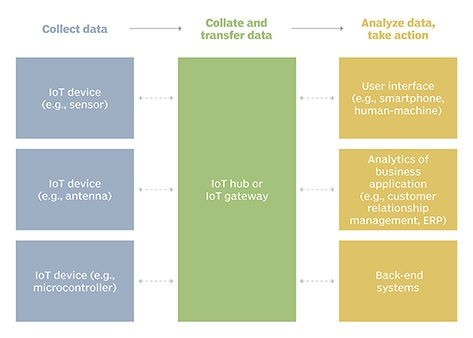
\includegraphics[height=9cm]{images/iot_system.jpg}
    \scriptsize{source :\url{https://internetofthingsagenda.techtarget.com/}}
    \caption{Exemple d'un systéme IoT}
    \label{fig:2.2}
\end{figure}
%%%%%%%%%%%%%%%%%%%%%%%%%%%%%%%%%%%%%%%%%%%%%%%%%%%%%%%%%%%%%%%%%%%%%%%
\subsection{Avantages du Big Data dans les composants de la ville intelligente}
\subsubsection{La smart gouvernance:}
La smart gouvernance soutient l'intégration et la collaboration de différentes agences gouvernementales et combine ou rationalise leurs processus. Cela se traduit par des opérations plus efficaces, un meilleur traitement des données partagées, une gestion et une application plus stricte de la réglementation.
Elle améliore les décisions commerciales grâce au support d'analyse Big Data. En recherchant le comportement et la croissance économique d’une entreprise en plus de ses concurrents et des conditions environnementales, les prises de décisions sont plus appropriées et plus efficaces en matière d’emploi, de production et de stratégies de localisation.
Elle permet la publication de nouvelles politiques au profit des propriétaires de données (citoyens) et des producteurs (agences gouvernementales). Les agences gouvernementales aident à développer la qualité des données, tandis que les citoyens montrent comment ils peuvent utiliser les données et les transférer vers de nouvelles connaissances afin d'améliorer la qualité des services publics.
Elle aident les gouvernements à se concentrer sur les préoccupations des citoyens en matière de santé et de protection sociale, de logement, d’éducation, de police et autres.\\
\subsubsection{Le smart environnement :}
Le smart environnement fournit des informations météorologiques qui permettront d’améliorer l’agriculture du pays, de mieux informer la population sur les conditions potentiellement dangereuses et de mieux gérer l’utilisation de l’énergie en fournissant des prévisions plus précises à la demande.\\
\subsubsection{La smart mobilité :}
La smart mobilité reconnaît les modèles de trafic en explorant les données en temps réel. 
Elle réduit les embouteillages sur les routes principales de la ville en prévoyant les conditions de circulation et en ajustant les contrôles de circulation. Grâce au Big Data, la ville intelligente peut réduire le trafic et les accidents en ouvrant de nouvelles routes, en améliorant l'infrastructure en fonction des données de congestion et en collectant des informations sur le parking et les routes alternatives.
Elle réduit les déchets de la chaîne d'approvisionnement en associant les livraisons et en optimisant les mouvements d'expédition.
Elle active la transmission en continu des données pour traiter et communiquer aux conducteurs les informations sur le trafic collectées via des capteurs, des feux de signalisation intelligents et des dispositifs embarqués via des smartphones ou d'autres dispositifs de communication.
Les mégadonnées peuvent être utilisées pour envoyer des informations en retour à des entités spécifiques afin qu’elles prennent des mesures visant à atténuer ou à résoudre un problème de trafic.\\
\subsubsection{La smart énergie:}
La smart énergie facilite la prise de décision concernant les niveaux d'approvisionnement en électricité en adéquation avec la demande réelle des citoyens et dans toutes les conditions qui affectent.
Elle permet la prévision en temps quasi réel grâce à une analyse efficace des données volumineuses collectées.
Elle s’aligne sur les objectifs stratégiques (optimisation des ressources) par le biais de plans de tarification spécifiques compatibles avec les modèles d'approvisionnement, de demande et de production.\\
\subsubsection{La smart éducation:}
La smart éducation optimise la recherche universitaire. Par exemple, l'astronome peut maintenant analyser un grand ensemble de données astronomiques en utilisant des ordinateurs puissants au lieu d'analyses manuelles. En analysant et en explorant des images numériques de haute qualité prises depuis l'espace, de nouvelles découvertes peuvent se produire sur le terrain. Cela s'applique à de nombreux domaines scientifiques et de recherche tels que les expériences médicales, les opérations de fabrication, les études environnementales et les analyses économiques et financières.
Le comportement et le jumelage mèneront à de nouvelles connaissances. De l'évaluation des diplômés aux attitudes en ligne, chaque élève génère un suivi de données unique. En analysant ces données, les établissements d’enseignement peuvent déterminer s’ils utilisent leurs ressources aux bons endroits et produisent les bons résultats.\\
\subsubsection{La smart sécurité:}
La smart sécurité fournit des cartes des zones géographiques détaillées sur le plan spatial et le plan temprel, permettant ainsi d’aider à déterminer facilement les changements qui pourraient survenir.
Elle aide à prévoir les changements environnementaux futurs ou les catastrophes naturelles telles que la détection des tremblements de terre, qui permettront de sauver des vies et d'économiser des ressources.\\

\subsection{Les exigences des applications de ville intelligente basées sur le Big Data}
Les applications de ville intelligente basées sur le Big Data doivent répondre à plusieurs exigences découlant de la nature particulière des besoins de la ville intelligente et des caractéristiques du Big Data. Certaines exigences sont technologiques, tandis que d’autres sont liées à la sensibilisation des citoyens et aux rôles des gouvernements.\\
\subsubsection{Gestion des données volumineuses : }
Le principal avantage des applications de ville intelligente est qu’elles génèrent de gros volumes de données dans divers formats et dans de nombreux secteurs tels que le trafic, l’énergie, l’éducation, la santé et la fabrication. Ces données sont générées et collectées de manière massive et régulière, offrant ainsi une vue en temps réel de ce qui se passe dans la ville à tout moment. Pour garantir une utilisation appropriée et utile de ces données dans les applications de ville intelligente, il est important de disposer d'outils de gestion des données volumineuses appropriés et efficaces. La gestion des données volumineuses comprend le développement et l'exécution d'architectures, de politiques, de pratiques et de procédures qui gèrent correctement l'ensemble du cycle de vie des données tout au long de son utilisation dans les applications de ville intelligente. Comme les données proviennent de sources différentes avec des formats différents, il est nécessaire de disposer de fonctionnalités avancées de gestion des données permettant de reconnaître les différents formats et sources de données, de structurer, de gérer, de classer et de contrôler tous ces types et structures. La gestion des données volumineuses pour les applications de ville intelligente doit également permettre une gestion évolutive de données volumineuses afin de prendre en charge les applications hors ligne, ainsi qu'un traitement à faible temps de latence pour servir efficacement les applications en temps réel.\\
\subsubsection{Plateformes de traitement de données volumineuses:}
Les applications Big Data pour les villes intelligentes doivent effectuer des analyses de données qui nécessitent généralement une capacité de traitement énorme. Cela conduit à la nécessité de disposer des plateformes matérielles et logicielles évolutives et fiables. Les plateformes logicielles pour les villes intelligentes doivent offrir des capacités de calcul hautes performances, être optimisées pour le matériel utilisé, être stables et fiables pour les différentes applications nécessitant des données en cours d'exécution, prendre en charge le traitement de flux, fournir des niveaux élevés de résilience aux pannes et soutenu par une équipe et un fournisseur bien formés et compétents. Il existe différentes plateformes logicielles d'analyse des données volumineuses, telles que Hadoop Mapreduce , HPCC, Stratosphere et IBM Infosphere Streams, qui fournissent le traitement de flux requis par les applications de données volumineuses en temps réel. Ces plateformes fonctionnent bien sur des systèmes en cluster capables de fournir une plateforme matérielle, puissante et évolutive pour répondre aux exigences des applications de données volumineuses. Les mégadonnées peuvent également être traitées sur le Cloud en utilisant à la fois une plateforme Big Data (PaaS) et une infrastructure IaaS.\\
\subsubsection{Infrastructure de réseau intelligent:}

La plupart des applications Big Data pour les villes intelligentes exigent des réseaux intelligents connectant leurs composants, y compris les équipements des résidents, tels que les voitures, les appareils intelligents et les téléphones intelligents. Ce réseau doit être capable de transférer efficacement les données collectées de leurs sources vers le lieu de collecte, de stockage et de traitement des données volumineuses, ainsi que de renvoyer les réponses aux différentes entités qui en ont besoin dans la ville intelligente. La prise en charge de la qualité de service (QoS) sur le réseau est extrêmement importante pour les applications Big Data en temps réel destinées aux villes intelligentes. \\
\subsubsection{Algorithmes avancés:}
Les algorithmes standards utilisés dans les applications classiques peuvent ne pas être suffisants ou efficaces pour gérer les applications de données volumineuses en raison de leurs exigences spécifiques et de la nécessité impérieuse d'un traitement à grande vitesse et à haut volume. Les applications de données volumineuses pour les villes intelligentes doivent mettre en œuvre des algorithmes avancés et plus sophistiqués pour traiter efficacement les données volumineuses. Certains de ces algorithmes doivent être conçus pour la prise en charge d'applications en temps réel, tandis que d'autres peuvent être conçus pour un traitement par lots ou hors ligne. Ces algorithmes doivent être optimisés pour gérer des volumes de données élevés, une grande variété de types de données, des contraintes de temps sur les processus de prise de décision et des composants distribués sur divers emplacements géographiques. De plus, ces algorithmes doivent fonctionner efficacement dans des environnements hétérogènes et être capables de gérer et de fonctionner dans des environnements hautement dynamiques.\\
\subsubsection{Sécurité et confidentialité:}
Étant donné que la plupart des données collectées et traitées dans les applications de ville intelligente contiennent une forme d’information confidentielle, il est important de veiller à ce que tous les composants de la technologie et des applications incluent et maintiennent des niveaux acceptables de mécanismes de sécurité et de confidentialité. Bien qu'une ville intelligente offre de nombreux avantages positifs à ses résidents, elle fait peser de nombreuses menaces sur leur sécurité, leur bien-être et leur vie privée en s'appuyant fortement sur leurs données. La possibilité d'accès illégal ou d'attaques malveillantes à de telles infrastructures peut entraîner des résultats catastrophiques pour l'infrastructure de la ville, ses entités gouvernementales et ses résidents. Les concepteurs et les développeurs d’applications Big Data doivent inclure les politiques et les procédures de sécurité et de confidentialité, dans la conception et la mise en œuvre de leurs applications. \\
\subsubsection{Sensibilisation des citoyens:}
Les citoyens doivent savoir utiliser correctement et en toute sécurité les solutions TIC pour une ville intelligente. Leur participation active au gain d'informations sur les différents problèmes rencontrés avec les applications de ville intelligente contribue à améliorer la qualité des données collectées et la performance des applications. Un autre aspect important de la sensibilisation des citoyens est leur connaissance et leur usage de bonnes pratiques en matière de sécurité et de protection de la vie privée. \\
\subsubsection{Rôle du gouvernement:}
Les entités gouvernantes des villes intelligentes doivent établir des principes directeurs d'ouverture, de transparence, de participation et de collaboration afin de contrôler les échanges et le flux de données volumineuses [14]. Les gouvernements jouent un rôle essentiel dans une ville intelligente. Le gouvernement doit revoir et réajuster les politiques en matière d'informations et de données, en fonction des besoins, en mettant l'accent sur la confidentialité, la réutilisation des données, la précision des données, l'accès aux données, leur archivage et leur conservation [14]. 
Pour prendre en charge efficacement les applications de données volumineuses, le gouvernement des villes intelligentes doit établir un équilibre entre les utilisations bénéfiques des données et les préoccupations des particuliers en matière de vie privée, en abordant certains des concepts fondamentaux des lois sur la vie privée.\\


\section{Visualisation du Big Data }
\subsection{Context}
Les villes cherchent à devenir intelligentes en connectant les systèmes isolés des organismes municipaux et en installant des capteurs intelligents. Les administrateurs de la ville cherchent à exploiter les informations tirées des données des capteurs de l'Internet des objets (IoT), de systèmes de positionnement global (GPS), de smartphones et d'ordinateurs. 80\% de ces données sont des données sombres, ce qui signifie que les données sont non structurées pour transmettre un sens en soi.
Il est important de visualiser les données traitées pour découvrir les modèles et pour décider les prochaines étapes. Dans le but de faire ce processus efficacement, il est extrêmement important que les décideurs puissent visualiser et interagir avec les données.
Cela signifie qu'il est possible de supprimer la dépendance sur des experts en données de la boucle, ce qui signifie aussi que la plateforme de visualisation de données doit être interactive pour interagir avec les données, donc les idées deviennent visuellement évidentes dans le processus de découverte.

\subsection{L’importance de la visualisation du Big Data}
La visualisation de données, qui exploite la puissance de la réalité virtuelle, de la réalité augmentée et de l’apprentissage automatique, est une plateforme idéale pour la visualisation de flux de données IoT. La visualisation naturelle basée sur les gestes est non seulement intuitive, mais elle est également capable de montrer des données spatiales et temporelles complexes sur la réplique virtuelle d’un environnement, par exemple le modèle Google Earth ou le prototype 3D d’une ville.
La nouvelle technologie nous libère des cages de données à écran plat bidimensionnelles et nous permet de pénétrer dans nos données elles-mêmes en nous aidant à découvrir des informations grâce à un moyen de corrélation visuelle simpliste mais très puissant. Il n’est pas difficile de prendre des décisions avec la visualisation des données.
Plusieurs avantages plus spécifiques méritent d’être pris en compte. Voici quelques-uns des avantages les plus précieux de la visualisation de données volumineuses :
\subsubsection{1. Traiter rapidement de grandes quantités de données:}
Avec autant d’informations saisies, organisées et analysées, il y a tout simplement trop de données brutes pour que l’esprit humain moyen puisse les traiter à un rythme raisonnable. La visualisation de données volumineuses supprime le long processus de compréhension des données et permet aux utilisateurs de digérer rapidement des quantités de données volumineux et complexes. Ceci est souvent accompli par l’utilisation de tableaux de bord interactifs, présentés visuellement.
\subsubsection{2. Accéder aux données importantes en temps réel:}
Dans le monde des affaires au rythme rapide, chaque seconde compte. Les entreprises qui doivent s’appuyer sur des méthodes plus traditionnelles pour rassembler et affiner une grande quantité de données se retrouvent souvent avec des informations obsolètes. D'autre part, les meilleurs outils de visualisation de données volumineuses fonctionnent en temps réel et mettent constamment à jour les informations présentées. Ainsi, chaque fois qu'un utilisateur a besoin d'y accéder, il dispose toujours des données les plus récentes.
\subsubsection{3. Voir les liens entre les processus métier et les performances:}
Même si peu de dirigeants nieraient le fait que les processus et les activités opérationnels quotidiens d’une organisation aient un impact direct sur les performances globales de l’entreprise, il peut être difficile de voir exactement comment ces activités affectent le succès de la société. Les outils de visualisation de données volumineuses résolvent ce problème en permettant aux dirigeants de découvrir visuellement les relations cachées qui relient les processus quotidiens aux performances de l'entreprise.
\subsubsection{4. Raconter une histoire à travers des données:}
L'esprit humain a tendance à préférer traiter les informations de manière linéaire, c'est-à-dire qu'il aime voir les causes, les effets et les résolutions alignés de manière à raconter une histoire. En présentant les données de manière centrée visuellement, la visualisation de données volumineuses donne à l’information quelque chose qui lui manque généralement : un sentiment de progression. Cela rend la compréhension plus facile et l’utilisation aussi à utiliser pour les utilisateurs.

%%%%%%%%%%%%%%%%%%%%%%%%%%%%%%%%%%%%%%%%%%%%%%%%%%%%%%%%%%%%%%%%%%%%%%%%
\subsection{Les techniques de visualisation dans un contexte Big Data }
Pour le Big Data, la visualisation n’est pas simplement une fonctionnalité pratique, c’est une obligation. En effet, un utilisateur ne peut saisir à lui seul les données volumineuses et en constante augmentation. Plusieurs techniques de visualisation Big Data existent; celles-ci peuvent être à la fois spécifiques et non spécifiques.
\subsubsection{Graphiques bidimensionnelle :}
Le moyen le plus simple de montrer le développement d'un ou de plusieurs ensembles de données est un graphique. Les informations données par les graphiques diffèrent selon qu’ils sont des graphiques à barres et linéaires montrant la relation entre les éléments dans le temps, ou des graphiques en camembert illustrant les composantes ou les proportions entre les éléments d'un ensemble.
\subsubsection{1. Graphique à barres:}
Le graphique à barres classique utilise des barres horizontales ou verticales (graphique à colonnes) pour montrer des comparaisons numériques discrètes entre les catégories. Un axe du graphique montre les catégories spécifiques comparées et l'autre axe représente une échelle de valeurs discrètes.
Les graphiques en barres se distinguent des histogrammes, car ils ne présentent pas de développement continu sur un intervalle. Les données discrètes du graphique à barres sont des données catégoriques et répondent donc à la question de "combien ?" dans chaque catégorie.

\begin{figure}[!ht]
    \centering
    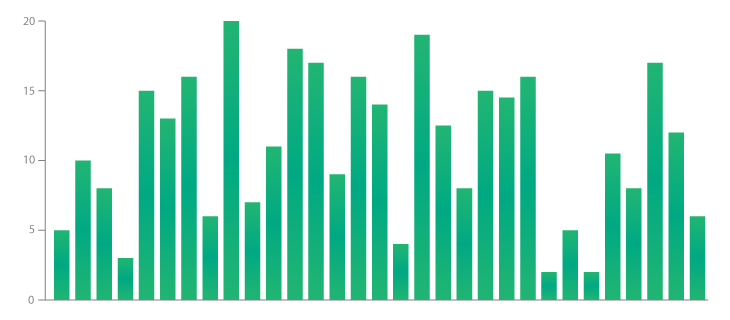
\includegraphics[height=5cm]{images/bar_chart.png}
    \scriptsize{source:\url{https://datavizcatalogue.com/methods/bar_chart.html}}
    \caption{Graphique à barres}
    \label{fig:2.3}
\end{figure}
\subsubsection{2.Camemberts }
\begin{wrapfigure}{R}{0.5\textwidth}
\centering
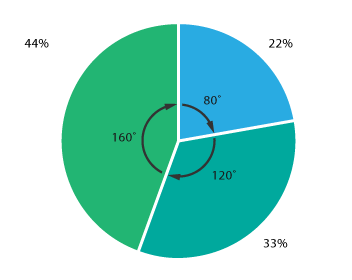
\includegraphics[width=0.4\textwidth]{images/pie_chart.png}
%\scriptsize{source :\url{https://datavizcatalogue.com/methods/pie_chart.html}}
\caption{\label{fig:2.4}Camemberts}
\end{wrapfigure}

Les camemberts aident à montrer les proportions et les pourcentages entre les catégories en divisant un cercle en segments proportionnels. Les entreprises qui utilisent à la fois des données traditionnelles et des données volumineuses peuvent utiliser cette technique pour examiner des segments de clientèle ou des parts de marché.
Chaque longueur d'arc représente une proportion de chaque catégorie, tandis que le cercle complet représente la somme totale de toutes les données, égale à 100\%.
Les camemberts sont idéaux pour donner au lecteur une idée rapide de la distribution proportionnelle des données.

\subsubsection{3. Graphiques linéaires}
Les graphiques linéaires sont utilisés pour afficher des valeurs quantitatives sur un intervalle ou une période continue. Le graphique linéaire est le plus souvent utilisé pour afficher les tendances et analyser l’évolution des données dans le temps.
Les graphiques linéaires sont dessinés en traçant d'abord les points de données sur une grille de coordonnées cartésiennes, puis en reliant une ligne entre tous ces points. En général, l'axe des ordonnées a une valeur quantitative, tandis que l'axe des abscisses est une échelle de temps ou une séquence d'intervalles. Les valeurs négatives peuvent être affichées sous l'axe des abscisses.
La direction des lignes sur le graphique fonctionne comme une belle métaphore pour les données: une pente ascendante indique où les valeurs ont augmenté et une pente descendante indique où les valeurs ont diminué. Le parcours de la ligne sur le graphique peut créer des modèles qui révèlent les tendances d'un jeu de données.
Lorsqu'elles sont regroupées avec d'autres lignes (autres séries de données), des lignes individuelles peuvent être comparées les unes aux autres. 
Dans la BI traditionnelle, les graphiques linéaires peuvent montrer l'évolution des ventes, des bénéfices et des revenus des 12 derniers mois. Lorsqu'elles utilisent le Big Data, les entreprises peuvent utiliser cette technique de visualisation pour suivre le nombre total de clics d'application par semaine, le nombre moyen de plaintes adressées au centre d'appels par mois, etc.
\begin{figure}[!ht]
    \centering
    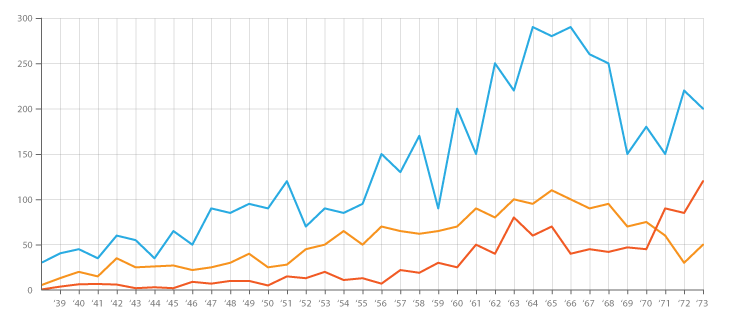
\includegraphics[height=5cm]{images/line_graph.png}
    \scriptsize{source :\url{https://datavizcatalogue.com/methods/pie_chart.html}}
    \caption{Graphique linéaire}
    \label{fig:2.5}
\end{figure}
Parmis les graphiques linéaires, il existe des graphiques en aires qui sont des graphiques en courbes, mais la zone située sous la ligne est remplie avec une certaine couleur. Les graphiques en aires sont dessinés en traçant d'abord les points de données sur une grille de coordonnées cartésiennes, en joignant une ligne entre les points et en remplissant l'espace situé en dessous de la ligne complétée.

\subsubsection{4.Diagramme de dispersion:}
Le diagramme de dispersion est également connu sous le nom de graphe de dispersion, de graphe de points, de tracé X-Y ou de Scattergramme.

Les diagrammes de dispersion utilisent une collection de points placés à l'aide de coordonnées cartésiennes pour afficher les valeurs de deux variables. En affichant une variable dans chaque axe, il est possible de détecter une relation ou une corrélation entre les deux variables.
\begin{figure}[!htb]
\begin{minipage}{0.46\linewidth}
Différents types de corrélation peuvent être interprétés à travers les modèles affichés sur les diagrammes de dispersion. Il existe une corrélation positive (les valeurs augmentent ensemble), négative (une valeur diminue avec l’augmentation), nulle (pas de corrélation), linéaire, exponentiel et en forme de U. La force de la corrélation peut être déterminée par la proximité des points sur le graphique. Les points qui finissent loin du groupe général de points sont appelés points aberrants.
Des lignes ou des courbes sont ajustées dans le graphique pour faciliter l'analyse et sont dessinées aussi près que possible de tous les points. Ainsi, il est montré comment tous les points ont été condensés en une seule droite. Ceci est généralement connu sous le nom de Droite de meilleur ajustement et peut être utilisé pour effectuer des estimations par interpolation.
Les diagrammes de dispersion sont parfaits lorsqu’il est associé des données numériques et que l’objectif est de voir si une variable a un impact sur l'autre. Cependant, il est important de rappeler que la corrélation n'est pas une cause et qu'une autre variable inaperçue peut influer sur les résultats.
\end{minipage}\hfil
\begin{minipage}{0.35\linewidth}
    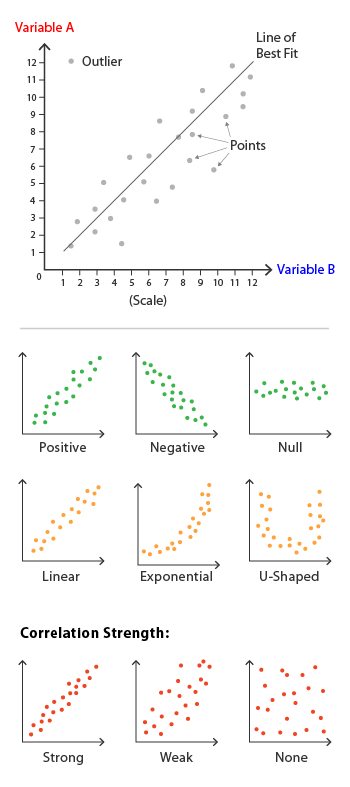
\includegraphics[height=13cm]{images/scatter-plot.png}
    \scriptsize{source :\url{https://datavizcatalogue.com/methods/scatterplot.html}}
    \caption{Diagramme de dispersion}
 \label{fig:4.6}
\end{minipage}
\end{figure}

\subsubsection{Techniques de visualisation des données géospatiales}
Les cartes sont largement utilisées dans différentes industries. Ils permettent de positionner des éléments sur des objets et des zones pertinents - cartes géographiques, plans de construction, aménagements de sites Web, etc. Parmi les visualisations de cartes les plus populaires, on compte les cartes thermiques, les cartes de distribution de points, les cartogrammes.

Parmis les techniques de visualisation des données géospatiales, il existe : 
\subsubsection{1. Les cartes à points (Dot Map)}
Les cartes à points sont un moyen de détecter les modèles spatiaux ou la distribution des données sur une région géographique, en plaçant des points de taille égale sur une région géographique.
Il existe deux types de cartes à points : un en un (un point représente un seul compte ou un objet) et un en plusieurs (un point représente une unité particulière, par exemple 1 point = 10 arbres).
Les cartes à points sont idéales pour voir comment les choses sont réparties sur une région géographique et peuvent révéler des motifs lorsque les points se regroupent sur la carte. Les cartes à points sont faciles à comprendre et donnent un meilleur aperçu des données, mais ne sont pas très utiles pour récupérer des valeurs exactes.
\begin{figure}[!ht]
    \centering
    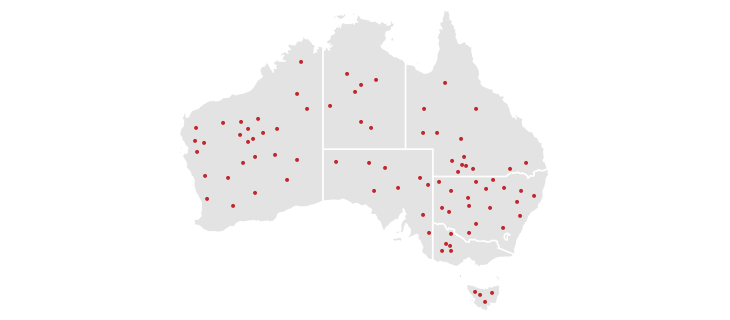
\includegraphics[height=5cm]{images/dot_map.png}
    \scriptsize{source :\url{https://datavizcatalogue.com/methods/dot_map.html}}
    \caption{Carte à point}
    \label{fig:2.7}
\end{figure}
\subsubsection{2. Les cartes à bulle (Bubble Map)}
Avec cette carte de données, les cercles sont affichés sur une région géographique désignée, la surface du cercle étant proportionnelle à sa valeur dans le jeu de données. Les cartes à bulles permettent de comparer des proportions sur des régions géographiques sans les problèmes causés par la taille de la région, comme le montre la carte de Choropleth. Cependant, l'un des principaux défauts de la carte à bulle est que des bulles trop volumineuses peuvent chevaucher d'autres bulles et régions sur la carte. Il faut donc en tenir compte.
\begin{figure}[!ht]
    \centering
    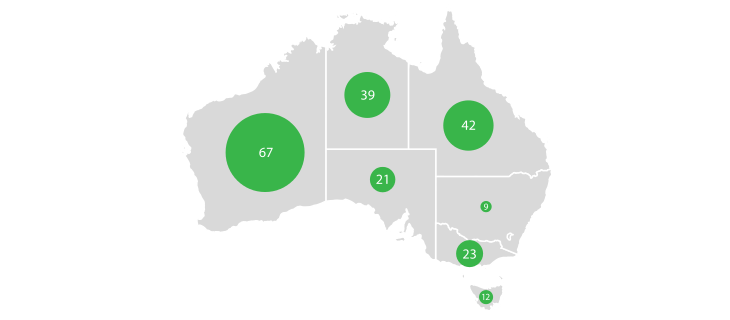
\includegraphics[height=5cm]{images/bubble_map.png}
    \scriptsize{source :\url{https://datavizcatalogue.com/methods/bubble_map.html}}
    \caption{Carte à bulle}
    \label{fig:2.8}
\end{figure}
\subsubsection{3. Les cartes Choroplèthes (Choropleth Map)}
Les cartes Choroplèthes affichent des zones géographiques ou des régions divisées colorées, ombrées ou structurées par rapport à une variable de données. Cela fournit un moyen de visualiser les valeurs sur une zone géographique, ce qui peut montrer des variations ou des modèles sur l'emplacement affiché.
La variable de données utilise la progression de la couleur pour se représenter dans chaque région de la carte. En règle générale, il peut s'agir d'un mélange d'une couleur à une autre, d'une progression de teinte unique, transparente à opaque, claire à sombre ou d'un spectre de couleurs complet.
\begin{figure}[!ht]
    \centering
    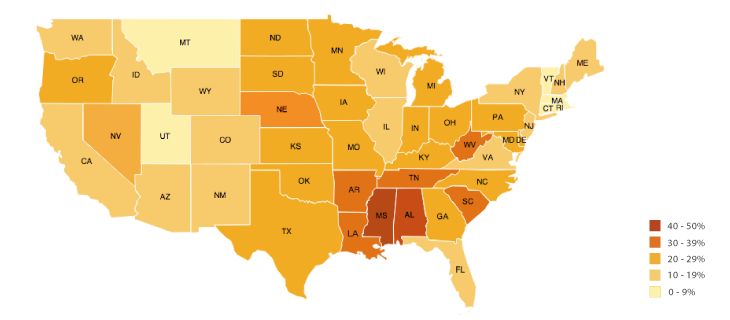
\includegraphics[height=5cm]{images/choropleth.png}
    \scriptsize{source :\url{https://datavizcatalogue.com/methods/choropleth.html}}
    \caption{Carte Choroplèthes 1}
    \label{fig:1.9}
\end{figure}

\begin{figure}[!htb]
\begin{minipage}{0.46\linewidth}
Un inconvénient de l'utilisation de la couleur est qu’il n’est pas possible de lire ou comparer avec précision les valeurs de la carte. Un autre problème est que les grandes régions apparaissent plus accentuées que les plus petites, ce qui affecte la perception des valeurs ombragées par l’utilisateur. 

Une erreur courante lors de la production de cartes Choroplèthes est de coder des valeurs de données brutes (telles que la population) plutôt que d'utiliser des valeurs normalisées (calcul de la population par kilomètre carré, par exemple) pour produire une carte de densité.
\end{minipage}\hfil
\begin{minipage}{0.35\linewidth}
    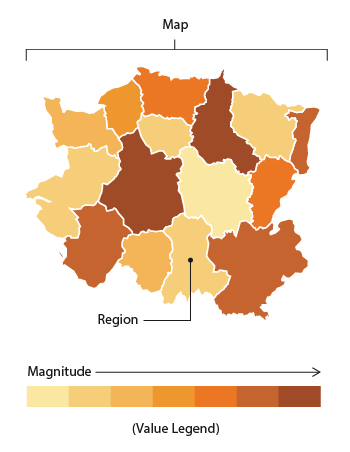
\includegraphics[height=8cm]{images/choropleth-zoom.png}
    \caption{Carte Choroplèthes 1}
 \label{fig:2.9}
\end{minipage}
\end{figure}
\subsubsection{4. Les cartes thermiques (Heatmap)}
La figure ~\ref{fig:2.11} ci-dessous montre les précipitations annuelles moyennes en Inde, en utilisant différentes nuances de bleu. Plus la nuance de bleu est sombre, plus les précipitations sont élevées.
\begin{wrapfigure}{R}{0.5\textwidth}
\centering
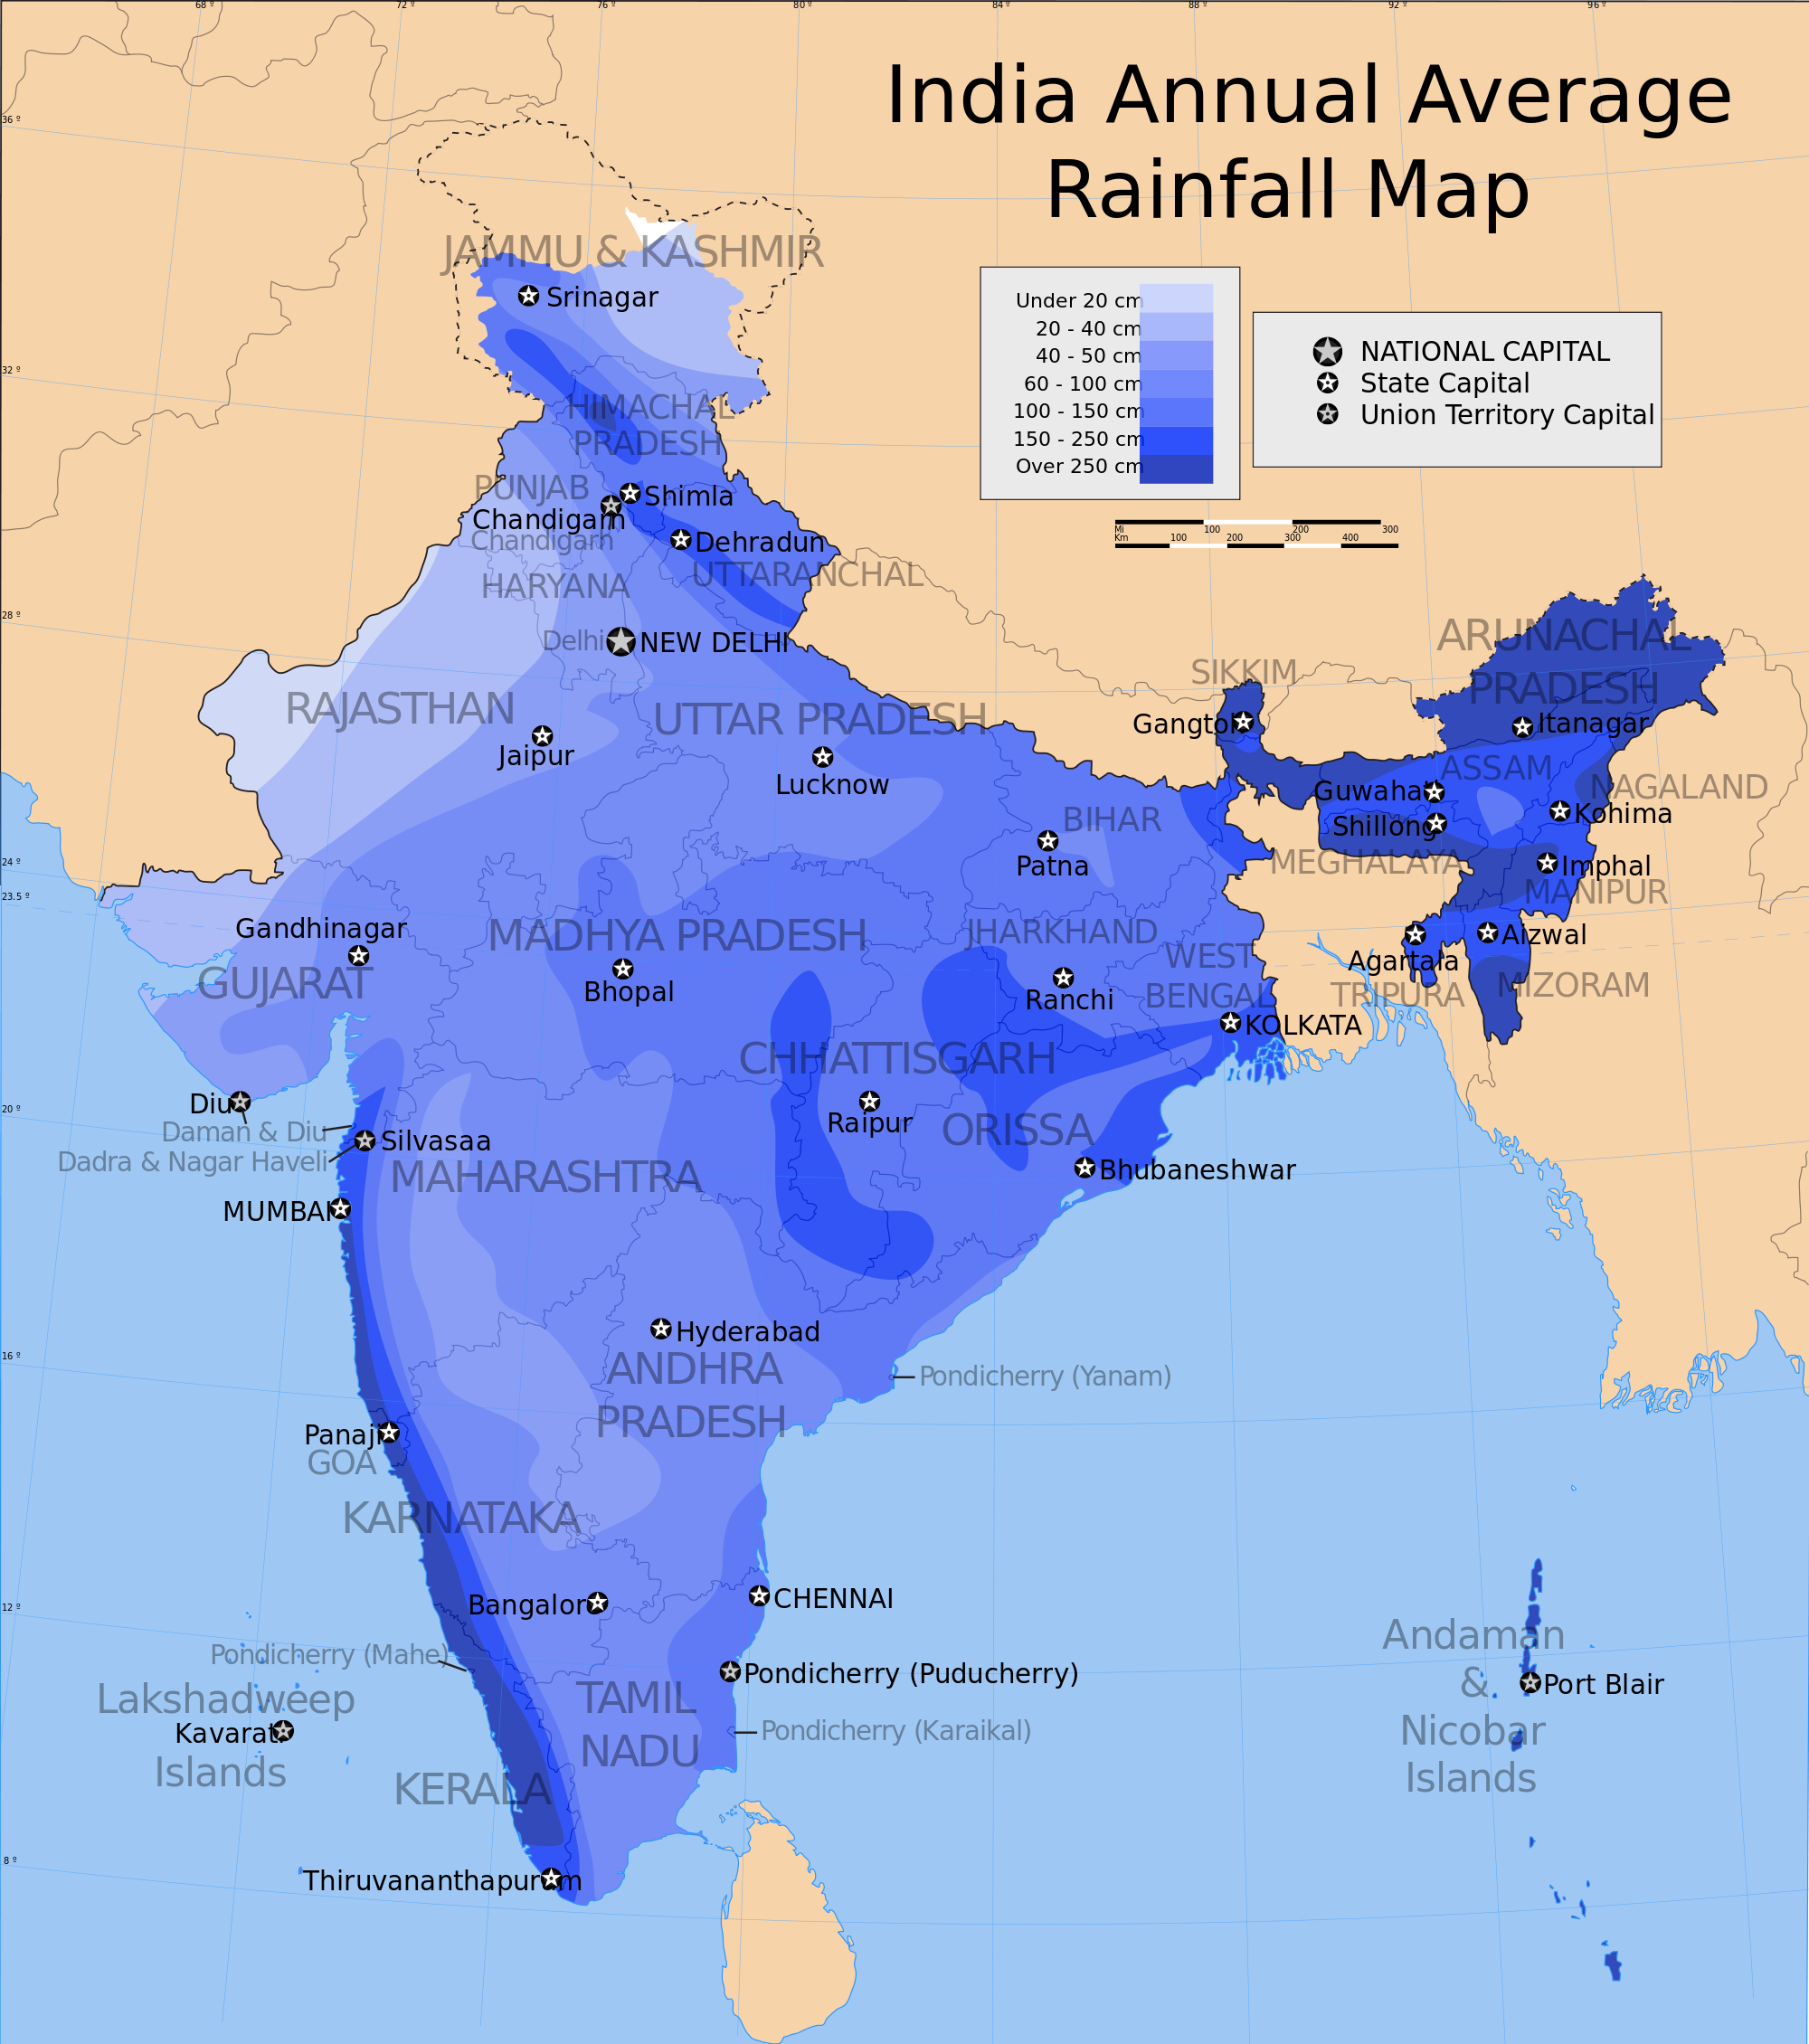
\includegraphics[width=0.4\textwidth]{images/Heatmap.png}
\scriptsize{source :\url{https://blog.socialcops.com/academy/resources/7-techniques-to-visualize-geospatial-data/}}
\caption{\label{fig:2.10} Carte thermique}
\end{wrapfigure}
Les cartes thermiques permettent de visualiser les données à travers des variations de coloration. Lorsqu'elles sont appliquées à un format tabulaire, les cartes thermiques sont utiles pour effectuer un examen croisé des données multivariées, en plaçant des variables dans les lignes et les colonnes, et en colorant les cellules du tableau. Les cartes thermiques sont utiles pour afficher la variance entre plusieurs variables, révéler toutes les tendances, indiquer si des variables sont similaires les unes aux autres et pour détecter si des corrélations existent entre elles. \\

En règle générale, toutes les lignes constituent une catégorie (étiquettes affichées à gauche ou à droite) et toutes les colonnes constituent une autre catégorie (étiquettes affichées en haut ou en bas). Les lignes et les colonnes individuelles sont divisées en sous-catégories, qui correspondent toutes les unes aux autres dans une matrice. Les cellules contenues dans le tableau contiennent des données catégoriques à code de couleurs ou des données numériques, basées sur une échelle de couleurs. Les données contenues dans une cellule sont basées sur la relation entre les deux variables de la ligne et de la colonne de connexion.

Une légende est nécessaire à côté d’une carte thermique pour que celle-ci puisse être lue avec succès. Les données catégorielles sont codées par couleur, tandis que les données numériques nécessitent une échelle de couleurs qui se mélange d'une couleur à l'autre afin de représenter la différence entre les valeurs hautes et basses. Une sélection de couleurs unies peut être utilisée pour représenter plusieurs plages de valeurs (0-10, 11-20, 21-30, etc.) ou vous pouvez utiliser une échelle de dégradé pour une seule plage (par exemple, 0 à 100) en mélangeant deux ou plus de couleurs ensemble.

En raison de leur confiance dans la couleur pour communiquer les valeurs, les Heatmaps sont un graphique mieux adapté pour afficher une vue plus générale des données numériques, car il est plus difficile de distinguer avec précision les différences entre les nuances de couleur et d’extraire des points de données spécifiques (à inclure les données brutes dans les cellules).
Les cartes thermiques peuvent également être utilisées pour afficher les modifications des données au fil du temps si l'une des lignes ou des colonnes est définie sur des intervalles de temps. Par exemple, utilisez une carte thermique pour comparer les changements de température au cours de l’année dans plusieurs villes, afin de déterminer les endroits les plus chauds ou les plus froids. Ainsi, les lignes pourraient répertorier les villes à comparer, les colonnes contiennent chaque mois et les cellules contiennent les valeurs de température.

\subsubsection{La Géovisualisation}
La géovisualisation est un terme court pour «Visualisation géographique» et désigne un ensemble d’outils et de techniques permettant d’appuyer l’analyse de données géospatiales au moyen de la visualisation interactive. A l'instar des domaines connexes de la visualisation scientifique et de la visualisation d'informations, la géovisualisation met l'accent sur la transmission d'informations. La géovisualisation communique les informations géospatiales d'une manière qui, associée à la compréhension humaine, permet l'exploration des données et la prise de décisions. Les cartes statiques traditionnelles ont une capacité d'exploration limitée; La géovisualisation permet des cartes plus interactives, y compris la possibilité d'explorer différentes couches de la carte, d'effectuer un zoom avant ou arrière et de modifier l'aspect visuel de la carte. La géovisualisation représente un ensemble de technologies et de pratiques cartographiques qui tirent parti de la capacité des technologies modernes d’apporter des modifications à une carte en temps réel, permettant aux utilisateurs d’ajuster les données cartographiées. Il est important de rendre les données complexes plus claires et utiles grâce à une conception visuelle appropriée, par exemple en inventant de nouvelles métaphores visuelles, en créant des algorithmes d'analyse, etc.
L'analyse visuelle intègre de nouveaux outils avec des techniques interactives innovantes et des représentations visuelles pour permettre une interaction homme-information. La conception des outils et des techniques repose sur des principes cognitifs et perceptuels. Cette science du raisonnement analytique fournit le cadre sur lequel on peut construire des technologies d'analyse visuelle stratégiques et tactiques pour l'analyse des menaces, la prévention et la réaction.
Les outils d'analyse visuelle doivent permettre différentes tâches d'analyse, telles que:
\begin{itemize}
\item Comprendre rapidement les situations, ainsi que les tendances et les événements qui ont généré les conditions actuelles.
\item Identifier les futurs possibles et leurs signes avant-coureurs
\item Surveiller les événements actuels pour détecter l'apparition de signes avant-coureurs et d'événements imprévus.
\end{itemize}

La gestion des données spatiales joue un rôle fondamental dans la conception de l’information urbaine, qui fait partie du cycle vertueux de l’information. La conception de l'information urbaine est l'un des outils les plus importants dans l'analyse des processus urbains et dans la planification d'une «ville intelligente».

Ces dernières années, différentes techniques de représentation des données spatiales ont été considérablement développées dans différents types de cartes (cartes de points, de lignes, de polygones, de cartes choroplètes, de cartes isoplètes, de cartogrammes, etc.). Les indicateurs spatiaux peuvent être représentés de différentes manières: en deux ou en trois dimensions, en fonction du caractère bidimensionnel ou tridimensionnel des phénomènes. Si le phénomène analysé a principalement deux dimensions, il est courant de le représenter en utilisant le même nombre de variables spatiales.
Un exemple des avantages obtenus en développant de nouvelles approches pour la cartographie des données en géovisualisation est illustré ci-dessous. La figure ~\ref{fig:1.12} présente les données sur les ventes des clients d'un établissement de vente au détail établi dans la région du Grand Toronto (GTA) utilisant une approche SIG traditionnelle. La figure ~\ref{fig:1.12} illustre le gain d'interprétation résultant de la cartographie 3D des mêmes données sous-jacentes. Le système SIG adapté utilisé dans cet exemple offre à l'utilisateur la possibilité de manipuler rapidement le niveau de déformation de l'axe Z et d'explorer la carte à partir de n'importe quelle perspective.
\begin{figure}[!ht]
    \centering
    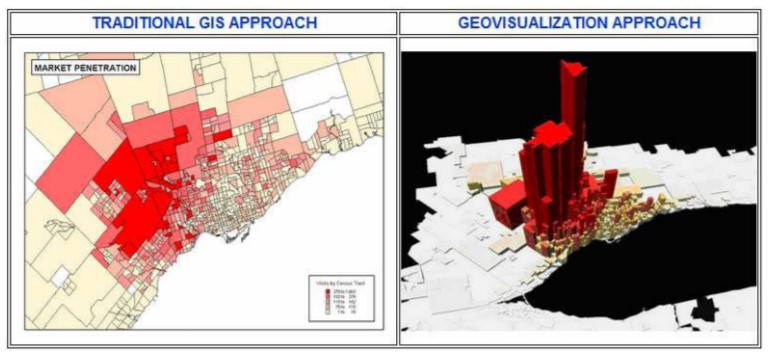
\includegraphics[height=5.5cm]{images/geo1.jpg}
    \scriptsize{source :\url{https://blog.socialcops.com/academy/resources/7-techniques-to-visualize-geospatial-data/}}
    \caption{La différence entre la visualisation par GIS traditionnel et la géovisualisation }
    \label{fig:1.12}
\end{figure}

%Les figures suivantes montrent quelques exemples de représentation spatiale de données et d'indicateurs dans les zones urbaines et extra-urbaines dans une approche SIG traditionnelle et dans une approche plus intéressante de la géovisualisation:
%\begin{figure}[!htp]
    %\centering
    %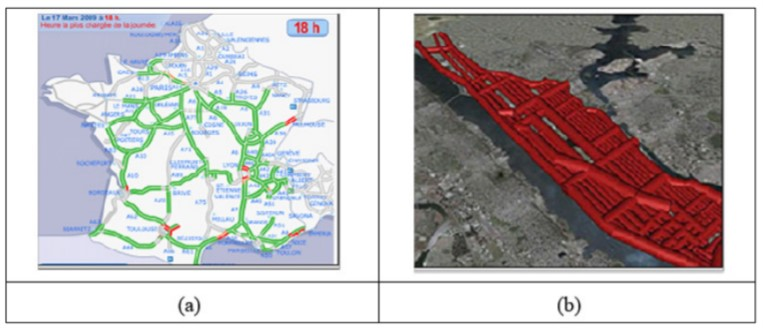
\includegraphics[height=5.5cm]{images/geo4.jpg}
    %\caption{Dans l'image de gauche (a), l'indicateur de la fluidité du trafic en deux dimensions en zone extra-urbaine, France (voir www.coraly.com);Dans l'image de droite (b), l'indicateur de flux de %trafic est affiché en trois jours.}
 %   \label{fig:2.13}
%\end{figure}

%\begin{figure}[!htp]
    %\centering
    %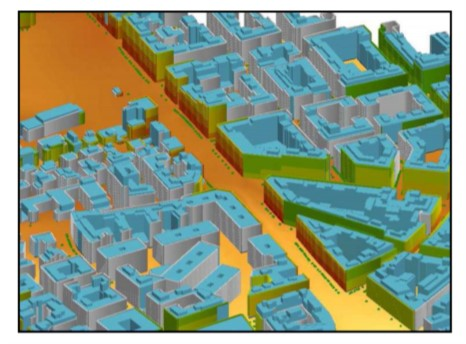
\includegraphics[height=5.5cm]{images/geo2.jpg}
    %\caption{Indicateur de température (ou de bruit) sur la façade de %bâtiments en milieu urbain [M. Ioannilli].}
 %   \label{fig:2.14}
%\end{figure}

%\begin{figure}[!htp]
    %\centering
   % 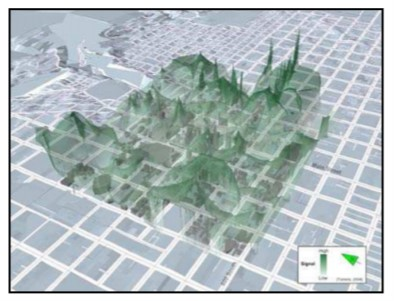
\includegraphics[height=5.5cm]{images/geo3.jpg}
  %  \caption{Indicateurs spatiaux: intensité du signal WI-FI d’Internet}
 %   \label{fig:2.15}
%\end{figure}
%%%%%%%%%%%%%%%%%%%%%%%%%%%%%%%%%%%%%%%%%%%%%%%%%%%%%%%%%%%%%%%%%%%%%%%%
\subsection{Outils de visualisation de données }
Les outils de visualisation de données sont exactement les armes dont nous avons besoin. Ces outils nous montrent diverses informations sur les données collectées. Les grands entreprises tels que Google et Microsoft collectent et manipulent des données volumineuses pour concevoir l'avenir de leurs stratégies commerciales. Dans cette section, nous discuterons de certains de ces outils de visualisation big data populaires.\\

\subsubsection{1. Google Chart}
Google est une référence évidente et est bien connu pour la convivialité offerte par ses produits et Google chart n’est pas une exception. C'est l'un des outils les plus simples pour visualiser de grands ensembles de données. Google chart contient un large éventail de galeries de graphiques, allant d'un simple graphique linéaire à une structure hiérarchique complexe en forme d'arborescence. Vous pouvez utiliser n'importe lequel de ces graphiques selon vos besoins. De plus, la partie la plus importante lors de la conception d’un graphique est la personnalisation et, avec Google, il est assez spartiate. Vous pouvez toujours demander de l’aide technique si vous voulez approfondir.
\begin{figure}[!htp]
    \centering
    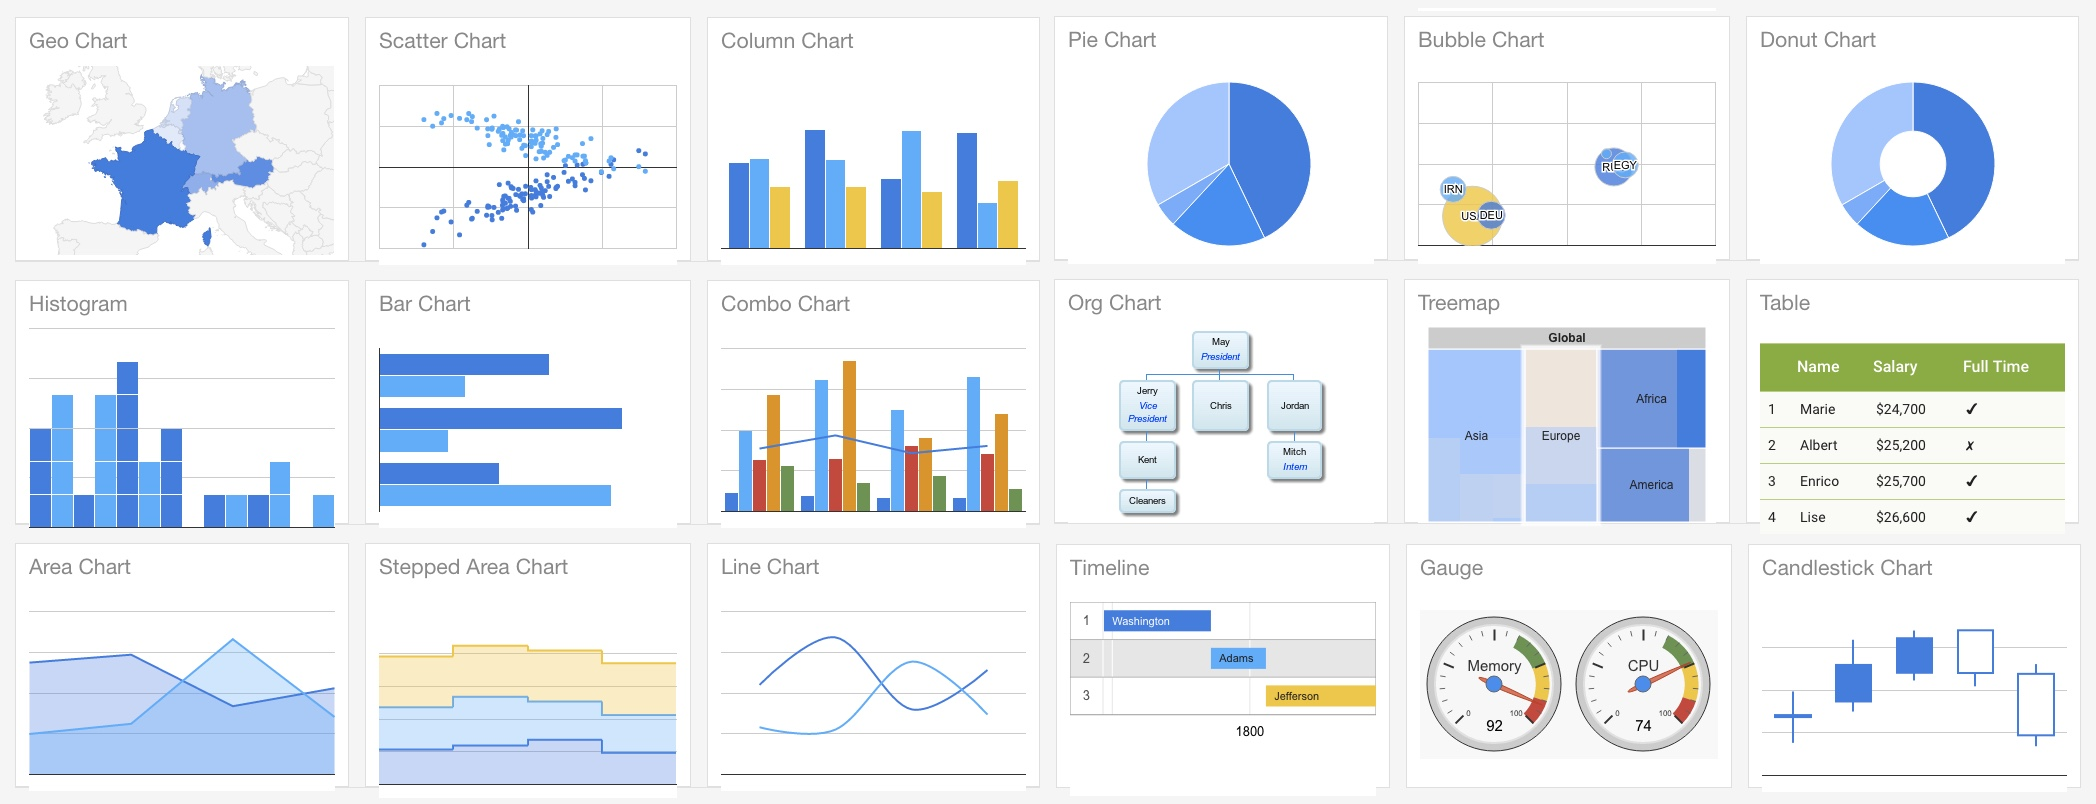
\includegraphics[height=6cm]{images/googlecharts.jpg}
    \scriptsize{source : \url{https://developers.google.com/chart/}}
    \caption{Google charts}
    \label{fig:2.16}
\end{figure}
\subsubsection{2. Tableau Chart}
Tableau Desktop est un incroyable outil de visualisation de données (SaaS) permettant de manipuler le Big Data. Il est disponible pour tout le monde. Il propose deux autres variantes, «Tableau Server» et «Tableau Online» dans le cloud, spécialement conçues pour les organisations liées au Big Data.

Il n’est pas nécessaire d’être un codeur pour utiliser cet outil. Cet outil est très pratique et fournit une vitesse ultra rapide. La toile ou le tableau de bord est convivial et compatible «glisser-déposer». Par conséquent, il crée une atmosphère conviviale dans tout environnement de travail.
\begin{figure}[!htp]
    \centering
    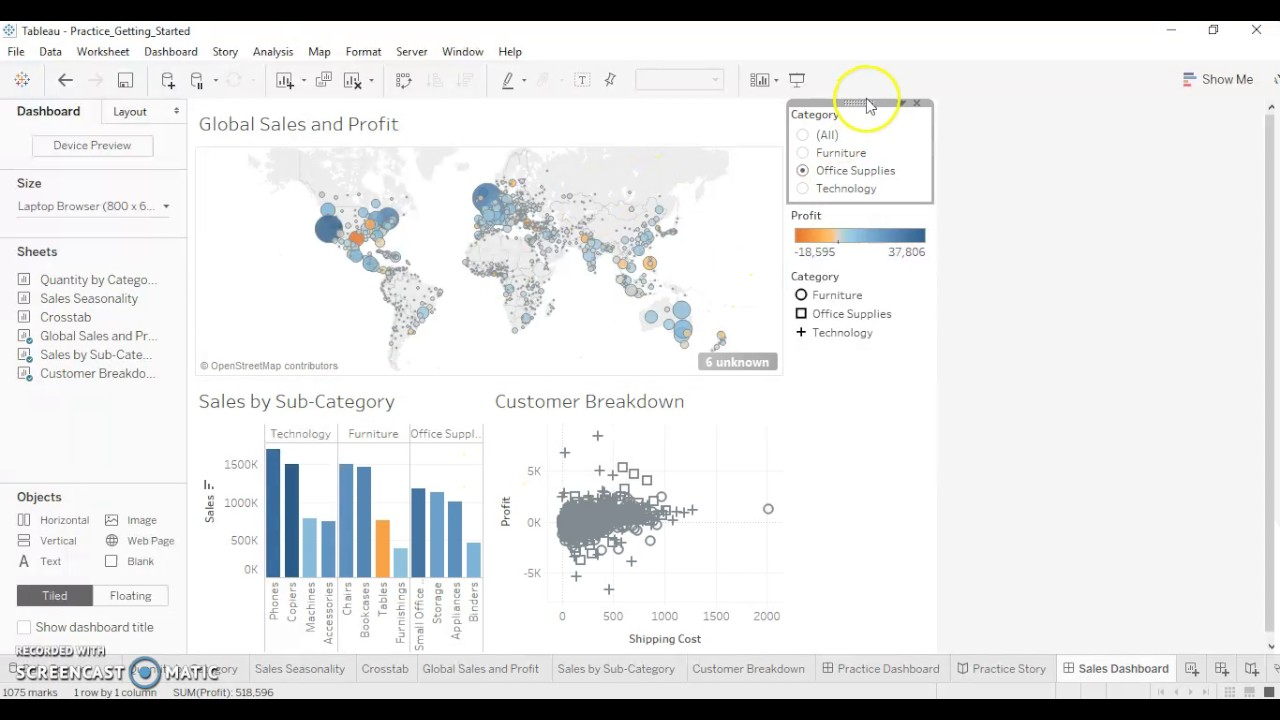
\includegraphics[height=8cm]{images/tableau.jpg}
    \scriptsize{source : \url{https://developers.google.com/chart/}}
    \caption{tableau charts}
    \label{fig:2.16}
\end{figure}
\subsubsection{3. D3js}
D3 ou Data Driven Document est une bibliothèque Javascript permettant de visualiser le Big Data de la manière que nous souhaitons. Ce n'est pas un outil, comme les autres, l'utilisateur a besoin de bien comprendre le javascript pour donner une forme aux données collectées. 

Intégrée à une page Web HTML, la bibliothèque JavaScript D3.js utilise des fonctions JavaScript prédéfinies pour sélectionner des éléments, créer des objets SVG, les styliser ou leur ajouter des transitions, des effets dynamiques ou des info-bulles. Ces objets peuvent également être largement stylisés à l'aide de CSS. Les grands ensembles de données peuvent facilement être liés à des objets SVG en utilisant de simples fonctions D3.js pour générer des graphiques et des diagrammes en texte enrichi / graphiques. Les données peuvent être sous différents formats, le plus souvent JSON, des valeurs séparées par une virgule (CSV) ou geoJSON, mais si nécessaire, des fonctions JavaScript peuvent être écrites pour lire d'autres formats de données.
D3.js est un projet open source et fonctionne sans plugin. Il nécessite très peu de code et présente les avantages suivants:
\begin{itemize}
    \item Excellente visualisation des données.
    \item C'est modulaire. Vous pouvez télécharger un petit fichier de D3.js que vous souhaitez utiliser.
    \item Pas besoin de charger toute la bibliothèque à chaque fois.
    \item Facile à construire un composant de cartographie.
    \item Manipulation DOM.
\end{itemize}
\subsubsection{Performance}
Étant donné que D3.js repose sur une série d’injecteurs (voir la section relative à l’architecture), la longueur et la complexité de la chaîne d’injection sont l’une des principales variables en termes de performances. Pour définir le coût d'une visualisation en termes de performances, vous devez mesurer certains aspects, tels que le temps de réponse (temps nécessaire pour traiter un seul élément), le débit (délai après le traitement d'un autre élément ou le "délai d'attente"). temps) et le temps de latence (le temps entre un changement dans le jeu de données et la première forme de sortie). Sur la base de ces métriques, il est possible de créer des solutions plus optimisées pouvant même tirer parti des modèles internes d’accélération.
Quatre composants principaux interviennent dans la chaîne de traitement de D3.js:
\begin{enumerate}
    \item Données d'entrée: ensemble d'entrées contenant les informations nécessaires à la création de la visualisation.
    \item Liaison d'élément: relation informelle entre une entrée de données et un élément dans le DOM.
    \item Chaîne de méthodes: la chaîne de méthodes qui extrait les paramètres d'élément en fonction des données.
    \item DOM (Document Object Model): éléments du document auxquels les entrées sont liées via la liaison d'élément.
    \item Ces processus sont plus faciles à comprendre lorsqu’ils sont visualisés comme dans l’image.
    
\end{enumerate}
\begin{figure}[!htp]
    \centering
    \includegraphics[height=3cm]{images/d3_diagram.png}
    \scriptsize{source : \url{https://delftswa.gitbooks.io/desosa2016/d3js/chapter.html}}
    \caption{D3 diagram}
    \label{fig:2.16}
\end{figure}

\subsubsection{Architecture}
D3.js étant un cadre avec lequel vous pouvez créer vos propres visualisations, il est principalement composé de fonctions et de modules qui créent des éléments dans une visualisation ou les modifient d’une manière ou d’une autre. La base est un module principal qui offre des méthodes de liaison document-données, dans lesquelles les autres modules se connectent pour créer les graphiques souhaités. En liant les éléments de données aux éléments du document, D3.js peut créer ces visualisations de manière transparente avec un temps système réduit. Le navigateur gère le rendu de la même manière qu’un document HTML / SVG classique et est donc très rapide.
L'architecture actuelle est basée sur des modules et des dépendances, qui sont visualisés dans l'image 5.
\begin{figure}[!htp]
    \centering
    \includegraphics[height=10cm]{images/d3_modules.png}
    \scriptsize{source : \url{https://delftswa.gitbooks.io/desosa2016/d3js/chapter.html}}
    \caption{D3 modules}
    \label{fig:2.16}
\end{figure}
D3 jouit d'une grande popularité avec une moyenne de 9 000 téléchargements [4] par semaine. Cette notoriété est le produit cumulatif d’une documentation et d’exemples détaillés, d’un excellent soutien de la part de la communauté et de l’approche facile de Michael Bostock lui-même. Le public cible est constitué d'un nombre toujours croissant de développeurs Web, de praticiens de la visualisation de données, de petites entreprises et de jeunes entreprises qui visent un grand bond en avant dans leurs connaissances et leur croissance. En conjonction avec ceux-ci, il existe divers géants du marché [2]. comme Microsoft (Microsoft BI utilise D3) qui ont utilisé D3 pour la visualisation interactive de données. Ce qui fait de D3 un choix attrayant pour de nombreuses entreprises, c’est sa flexibilité graphique dans la représentation des données et sa capacité à assumer divers rôles. Plusieurs outils, tels que des outils d'exploration, des outils d'exploration de données, des outils de communication et des outils d'analyse peuvent être conçus avec cette base. Ci-dessous sont les entreprises qui utilisent beaucoup D3.js dans les visualisations de médias, les reportages de mode et bien plus encore.

Open Street map: Éditer les plans des rues ouvertes
Dataviz: pour les outils de communication et de gestion
Chart.io: Fournir des solutions de tableau de bord professionnel
Plotly: Parcelles de rendu
DataMeer: Représenter l'exploration Big Data
New York Times: Graphes de rendu et analyse statistique.
%%%%%%%%%%%%%%%%%%%%%%%%%%%%%%%%%%%%%%%%%%%%%%%%%%%%%%%%%%%%%%%%%%%%%%%%%%%%%
\chapter{Quel est l'impact de la visualisation du Big Data sur les smart cities}
\section{Etude comparative }
L’objectif de cette partie est de réaliser une étude comarative entre les deffernet technique de la visualisation Big data :
\subsection{Selon des critères d'affaires}
\subsection{Selon des critères techniques}

\section{Les éléments déterminant le choix de visualisation du Big Data}
Mauvaises tactiques peuvent ne pas présenter tout le potentiel des données, ou même les rendre non pertinentes. Etudier le choix de technique ou les outiles de la visualisation big data selon (Public - Contenu - Le contexte - Dynamique - Objectif).
\section{Les défis de la visualisation du Big Data}
L’objectif de cette partie est d’aborder les difficultés et les défis de la visualisation du Big Data. 
\section{Défis et opportunités avec la visualisation du Big Data dans le contexte des Smart Cities}
L’objectif de cette partie est d’aborder les difficultées et les défis de la visualisation du Big Data dans le cadre d’une smart city. 

\chapter{Cas pratique: visualisation du Big Data chez Datategy}
\section{Presentation de Datategy}
DATATEGY est une société de conseil et d’expertise en Data Science. Elle conçoit, développe et commercialise une plateforme prédictive de lutte contre la fraude basée sur les technologies d’intelligence artificielle 100\% cloud......
\section{Presentation d’OctoCity solution}
La Smart City, ou ville intelligente consiste globalement en l’optimisation des coûts, de l’organisation, du bien-être des habitants.La ville est au service du citoyen mais ce dernier a néanmoins des obligations à respecter pour s’inscrire lui même comme acteur bénéficiant de ses services .Nous agissons en droite ligne avec l’objectif des opérateurs, des métropoles, et des territoires afin d’accompagner cet enjeu sociétal, politique et environnemental.Les solutions développées par DATATEGY s’interconnectent avec les réseaux existants, le croisement et l’exploitation des données.......
\section{Visualisation big data dans le cadre de la solution OctoCity}
L'objectif de cette partie est de présenter les tâches qui été réalisés sur la visualisation de Big data dans le cadre de la solution OctoCity.(état de l’art- Critiques - proposition et réflexion).

\subsubsection{Bublle map}
\begin{figure}[!htp]
    \centering
    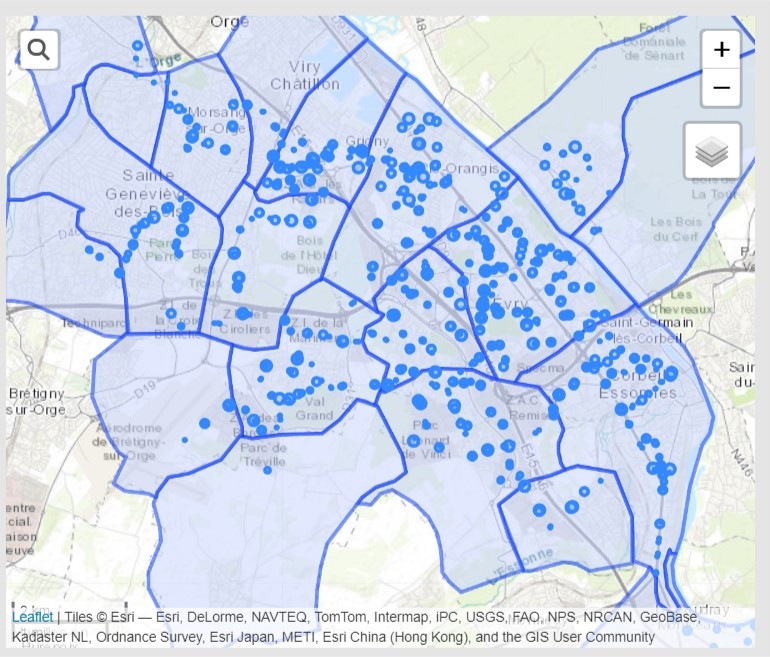
\includegraphics[height=6cm]{images/datategy-bubble-map.jpg}
    \scriptsize{}
    \caption{Visualisation le numbre de controle}
    \label{fig:3.1}
\end{figure}


\subsubsection{Scatter plot}
\begin{figure}[!htp]
    \centering
    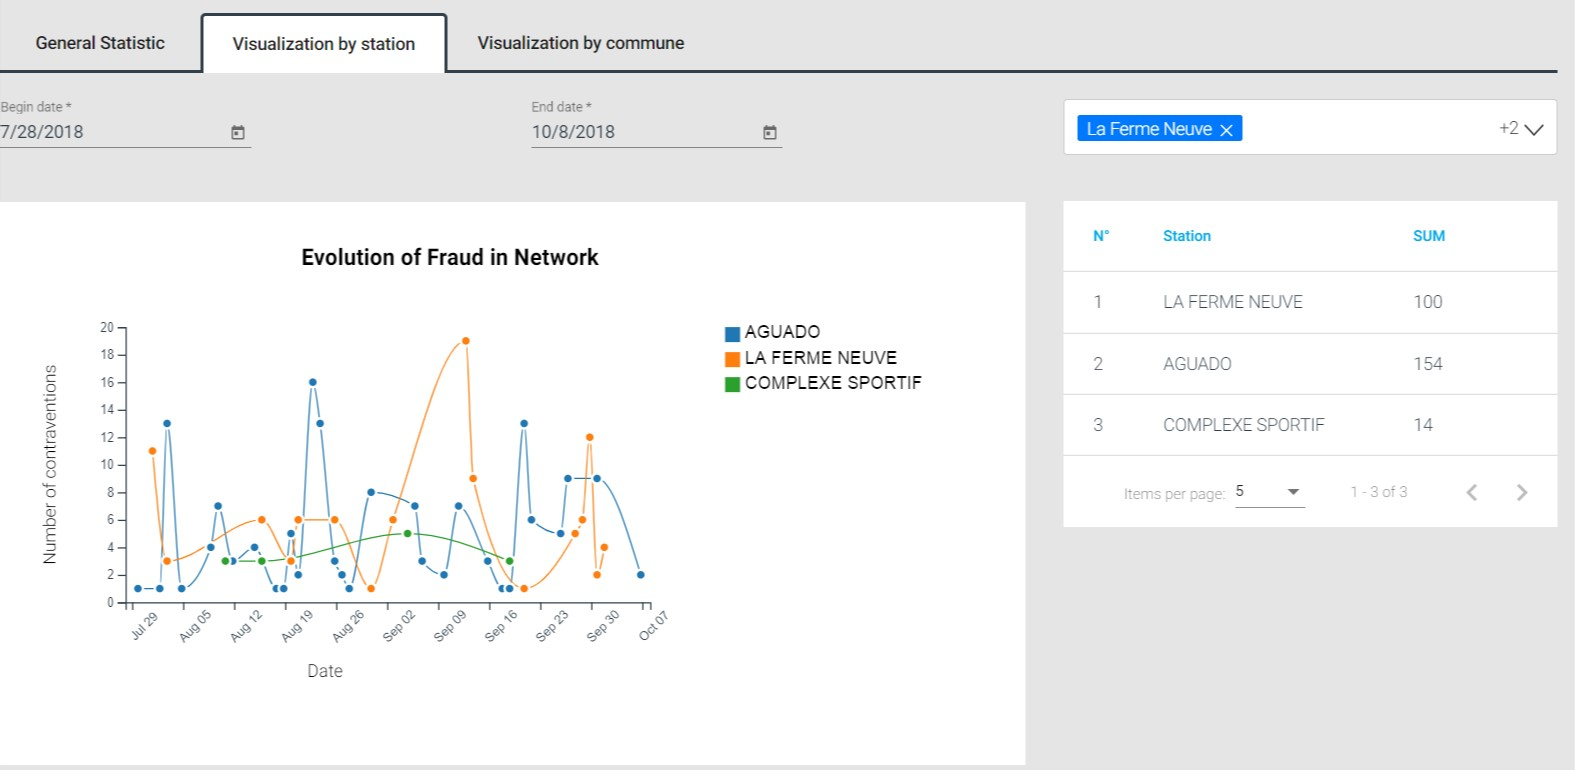
\includegraphics[height=6cm]{images/datategy-scatter-plot.jpg}
    \scriptsize{}
    \caption{Visualisation le numbre de contravention par station}
    \label{fig:3.2}
\end{figure}


\subsubsection{Suburst diagram}
\begin{figure}[!htp]
    \centering
    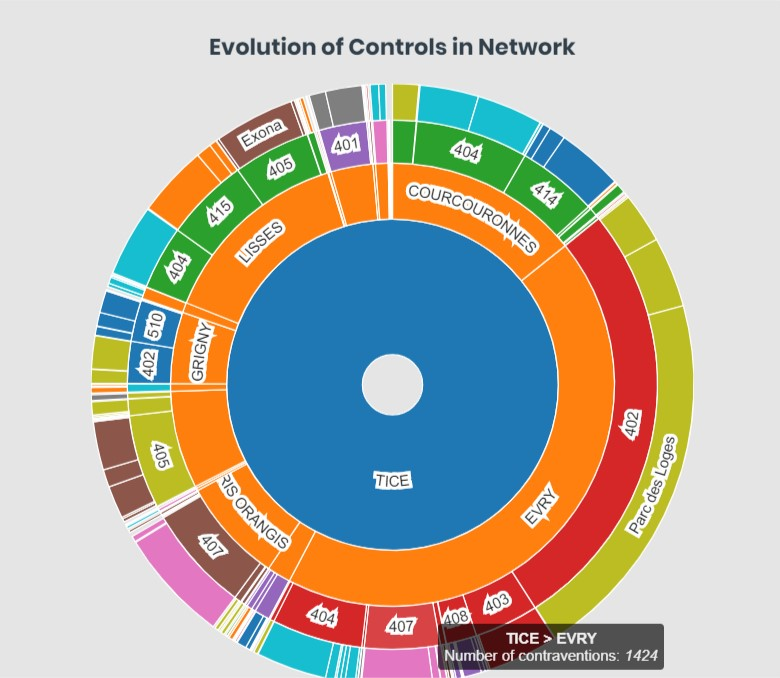
\includegraphics[height=6cm]{images/datategy-sunburst.jpg}
    \scriptsize{}
    \caption{Visualisation le numbre de contravention par 3 niveaux}
    \label{fig:3.3}
\end{figure}

\chapter{ Bilan et conclusion}
\section{Bilan professionnel}
\section{Bilan personnel}
\section{Conclusion}
En conclusion ...... 

% \nocite{*}
% \bibliographystyle{plain}
% \bibliography{biblio} 
% \phantomsection 
\addcontentsline{toc}{chapter}{Bibliographie} 
\begin{thebibliography}{9}
\bibitem{0}
United Nations. \emph{P.D.: The World’s Cities in 2016. United Nations}. [2016].

\bibitem{1} Neirotti \emph{, P., De Marco, A., Cagliano, A.C., Mangano, G., Scorrano, F.: Current trends in Smart City initiatives: some stylised facts. Cities 38, 25–36}. [2014]


\bibitem{2}  Liotine, M., Ramaprasad, \emph{, A., Syn, T.: Managing a Smart City’s resilience to Ebola: an ontological framework. In: 2016 49th Hawaii International Conference on System Sciences (HICSS), pp. 2935–2943. IEEE (2016)}. [2016]

\bibitem{3} Nam, T., Pardo\emph{, T.A.: Conceptualizing smart city with dimensions of technology, people, and institutions. In: Proceedings of the 12th Annual International Digital Government Research Conference: Digital Government Innovation in Challenging Times, pp. 282–291. ACM}.

\bibitem{4}IESE\emph{Ranking The World’s ‘Smartest’ Cities. Forbes. Forbes}. [2016]

\bibitem{5}Cameron, J.D., Ramaprasad, A., Syn,\emph{T.: An ontology of mHealth. Int. J. Med. Inform. 16–25}. [2017]

\bibitem{6} Murgante, B., Borruso,\emph{G.: Cities and smartness: the true challenge. Int. J. Agric. Environ. Inf. Syst. 6, 5}. [2015]

\bibitem{7}Khan Z, Anjum A, Kiani,\emph{SL. Cloud Based Big Data Analytics for Smart Future Cities. In Proceedings of the 2013 IEEE/ACM 6th International Conference on Utility and Cloud Computing. IEEE Computer Society; 2013. pp. 381–386.}



\end{thebibliography}
\end{document}
